\documentclass[3p,preprint,12pt]{elsarticle}
%\documentclass[preprint,12pt]{elsarticle}

\journal{Composites Part B: Engineering}

%%%%%%%%%%%%%%%%%%%%%%%
%% Elsevier bibliography styles
%%%%%%%%%%%%%%%%%%%%%%%
%% To change the style, put a % in front of the second line of the current style and
%% remove the % from the second line of the style you would like to use.
%%%%%%%%%%%%%%%%%%%%%%%

%% Numbered
%\bibliographystyle{model1-num-names}

%% Numbered without titles
%\bibliographystyle{model1a-num-names}

%% Harvard
%\bibliographystyle{model2-names} \biboptions{authoryear}

%% Vancouver numbered
\usepackage{numcompress}
\bibliographystyle{model3-num-names}

%% Vancouver name/year
%\usepackage{numcompress}\bibliographystyle{model4-names}\biboptions{authoryear}

%% APA style
%\bibliographystyle{model5-names}
%\biboptions{authoryear}

%% AMA style
%\usepackage{numcompress}\bibliographystyle{model6-num-names}

%% `Elsevier LaTeX' style
%\bibliographystyle{elsarticle-num}
\biboptions{sort&compress}
%\biboptions{longnamesfirst,angle,semicolon}
%%%%%%%%%%%%%%%%%%%%%%%


%\makeatletter
%\usepackage{wrapfig}
%\newcounter{aubio}
%
%\long\def\bioItem{%
%\@ifnextchar[{\@bioItem}{\@@bioItem}}
%
%\long\def\@bioItem[#1]#2#3{
% \stepcounter{aubio}
% \expandafter\gdef\csname authorImage\theaubio\endcsname{#1}
% \expandafter\gdef\csname authorName\theaubio\endcsname{#2}
% \expandafter\gdef\csname authorDetails\theaubio\endcsname{#3}
%}
%
%\long\def\@@bioItem#1#2{
% \stepcounter{aubio}
% \expandafter\gdef\csname authorName\theaubio\endcsname{#1}
% \expandafter\gdef\csname authorDetails\theaubio\endcsname{#2}
%}
%
%\newcommand{\checkheight}[1]{%
%  \par \penalty-100\begingroup%
%  \setbox8=\hbox{#1}%
%  \setlength{\dimen@}{\ht8}%
%  \dimen@ii\pagegoal \advance\dimen@ii-\pagetotal
%  \ifdim \dimen@>\dimen@ii
%    \break
%  \fi\endgroup}
%
%\def\printBio{%
%  \@tempcnta=0
%   \loop
%     \advance \@tempcnta by 1
%     \def\aubioCnt{\the\@tempcnta}
%     \setlength{\intextsep}{0pt}%
%     \setlength{\columnsep}{10pt}%
%     \expandafter\ifx\csname authorImage\aubioCnt\endcsname\relax%
%      \else%
%       \checkheight{\includegraphics[height=1.25in,width=1in,keepaspectratio]{\csname authorImage\aubioCnt\endcsname}}
%        \begin{wrapfigure}{l}{25mm}
%         \includegraphics[height=1.25in,width=1in,keepaspectratio]{\csname authorImage\aubioCnt\endcsname}%height=145pt
%        \end{wrapfigure}\par
%      \fi
%     \noindent\textbf{\csname authorName\aubioCnt\endcsname}\csname authorDetails\aubioCnt\endcsname \par\bigskip
%      \ifnum\@tempcnta < \theaubio
%   \repeat
%   }
%\makeatother

      

\usepackage{tabulary,xcolor}
\usepackage{amsfonts,amsmath,amssymb}
%\usepackage[T1]{fontenc}
%\makeatletter
%\let\save@ps@pprintTitle\ps@pprintTitle
%\def\ps@pprintTitle{\save@ps@pprintTitle\gdef\@oddfoot{\footnotesize\itshape \null\hfill\today}}
%\def\hlinewd#1{%
%  \noalign{\ifnum0=`}\fi\hrule \@height #1%
%  \futurelet\reserved@a\@xhline}
%\def\tbltoprule{\hlinewd{.8pt}\\[-12pt]}
%\def\tblbottomrule{\noalign{\vspace*{6pt}}\hline\noalign{\vspace*{2pt}}}
%\def\tblmidrule{\noalign{\vspace*{6pt}}\hline\noalign{\vspace*{2pt}}}
%\AtBeginDocument{\ifNAT@numbers \biboptions{sort&compress}\fi}
%\makeatother

  
%\renewenvironment{abstract}{\global\setbox\absbox=\vbox\bgroup
%  \hsize=\textwidth\def\baselinestretch{1}%
%\noindent\unskip\textbf{}
% \par\medskip\noindent\unskip\ignorespaces}
% {\egroup}
  

%\renewcommand{\bibnumfmt}[1]{{#1}.}

%\geometry{margin=3cm}
\linespread{1.5}

%\usepackage{fancyhdr}
%\fancypagestyle{headings}{\renewcommand{\headrulewidth}{0pt}\fancyhf{}\fancyfoot[R]{\thepage}}\pagestyle{headings}
%\fancypagestyle{pprintTitle}{\renewcommand{\headrulewidth}{0pt}\fancyhf{}\fancyfoot[R]{\thepage}}

%\usepackage{ifluatex}
%\ifluatex
%\usepackage{fontspec}
%\defaultfontfeatures{Ligatures=TeX}
%\usepackage[]{unicode-math}
%\unimathsetup{math-style=TeX}
%\else 
%\usepackage[utf8]{inputenc}
%\fi 
%\ifluatex\else\usepackage{stmaryrd}\fi

  
%%%%%%%%%%%%%%%%%%%%%%%%%%%%%%%%%%%%%%%%%%%%%%%%%%%%%%%%%%%%%%%%%%%%%%%%%%
% Following additional macros are required to function some 
% functions which are not available in the class used.
%%%%%%%%%%%%%%%%%%%%%%%%%%%%%%%%%%%%%%%%%%%%%%%%%%%%%%%%%%%%%%%%%%%%%%%%%%
\usepackage{url,multirow,morefloats,floatflt,cancel,tfrupee}
\makeatletter


\AtBeginDocument{\@ifpackageloaded{textcomp}{}{\usepackage{textcomp}}}
\makeatother
\usepackage{colortbl}
\usepackage{xcolor}
\usepackage{pifont}
\usepackage[nointegrals]{wasysym}
\urlstyle{rm}

\makeatletter
%%%For Table column width calculation.
\def\mcWidth#1{\csname TY@F#1\endcsname+\tabcolsep}

%%Hacking center and right align for table
\def\cAlignHack{\rightskip\@flushglue\leftskip\@flushglue\parindent\z@\parfillskip\z@skip}
\def\rAlignHack{\rightskip\z@skip\leftskip\@flushglue \parindent\z@\parfillskip\z@skip}


%\if@twocolumn\usepackage{dblfloatfix}\fi
\usepackage{ifxetex}
\ifxetex\else\if@twocolumn\usepackage{dblfloatfix}\fi\fi

\AtBeginDocument{
\expandafter\ifx\csname eqalign\endcsname\relax
\def\eqalign#1{\null\vcenter{\def\\{\cr}\openup\jot\m@th
  \ialign{\strut$\displaystyle{##}$\hfil&$\displaystyle{{}##}$\hfil
      \crcr#1\crcr}}\,}
\fi
}

%For fixing hardfail when unicode letters appear inside table with endfloat
\AtBeginDocument{%
  \@ifpackageloaded{endfloat}%
   {\renewcommand\efloat@iwrite[1]{\immediate\expandafter\protected@write\csname efloat@post#1\endcsname{}}}{\newif\ifefloat@tables}%
}%

\def\BreakURLText#1{\@tfor\brk@tempa:=#1\do{\brk@tempa\hskip0pt}}
\let\lt=<
\let\gt=>
\def\processVert{\ifmmode|\else\textbar\fi}
\let\processvert\processVert

\@ifundefined{subparagraph}{
\def\subparagraph{\@startsection{paragraph}{5}{2\parindent}{0ex plus 0.1ex minus 0.1ex}%
{0ex}{\normalfont\small\itshape}}%
}{}

% These are now gobbled, so won't appear in the PDF.
\newcommand\role[1]{\unskip}
\newcommand\aucollab[1]{\unskip}
  
\@ifundefined{tsGraphicsScaleX}{\gdef\tsGraphicsScaleX{1}}{}
\@ifundefined{tsGraphicsScaleY}{\gdef\tsGraphicsScaleY{.9}}{}
% To automatically resize figures to fit inside the text area
\def\checkGraphicsWidth{\ifdim\Gin@nat@width>\linewidth
	\tsGraphicsScaleX\linewidth\else\Gin@nat@width\fi}

\def\checkGraphicsHeight{\ifdim\Gin@nat@height>.9\textheight
	\tsGraphicsScaleY\textheight\else\Gin@nat@height\fi}

\def\fixFloatSize#1{}%\@ifundefined{processdelayedfloats}{\setbox0=\hbox{\includegraphics{#1}}\ifnum\wd0<\columnwidth\relax\renewenvironment{figure*}{\begin{figure}}{\end{figure}}\fi}{}}
\let\ts@includegraphics\includegraphics

\def\inlinegraphic[#1]#2{{\edef\@tempa{#1}\edef\baseline@shift{\ifx\@tempa\@empty0\else#1\fi}\edef\tempZ{\the\numexpr(\numexpr(\baseline@shift*\f@size/100))}\protect\raisebox{\tempZ pt}{\ts@includegraphics{#2}}}}

%\renewcommand{\includegraphics}[1]{\ts@includegraphics[width=\checkGraphicsWidth]{#1}}
\AtBeginDocument{\def\includegraphics{\@ifnextchar[{\ts@includegraphics}{\ts@includegraphics[width=\checkGraphicsWidth,height=\checkGraphicsHeight,keepaspectratio]}}}

\DeclareMathAlphabet{\mathpzc}{OT1}{pzc}{m}{it}

\def\URL#1#2{\@ifundefined{href}{#2}{\href{#1}{#2}}}

%%For url break
\def\UrlOrds{\do\*\do\-\do\~\do\'\do\"\do\-}%
\g@addto@macro{\UrlBreaks}{\UrlOrds}

\@ifundefined{quoteAttrib}
	{\long\def\quoteAttrib#1{\par\raggedleft\itshape#1\unskip}}
	{}

\@ifundefined{titlequoteAttrib}
	{\long\def\titlequoteAttrib#1{\list{}{\topsep-3pt\leftmargin.5in\rightmargin0pt}%
  \item\relax---\upshape#1\endlist}}{}

\renewenvironment{quote}
	{\list{}{\leftmargin.5in\rightmargin\leftmargin}%
  \item\relax}
  {\endlist}

\newenvironment{title-quote}
	{\list{}{\fontsize{10pt}{12pt}\selectfont\leftmargin.5in\itshape\rightmargin\leftmargin}%
  \item\relax}
  {\endlist}
\makeatother


%\def\floatpagefraction{0.8} 
%\def\dblfloatpagefraction{0.8}
%\def\style#1#2{#2}
%\def\xxxguillemotleft{\fontencoding{T1}\selectfont\guillemotleft}
%\def\xxxguillemotright{\fontencoding{T1}\selectfont\guillemotright}
%%%%%%%%%%%%%%%%%%%%%%%%%%%%%%%%%%%%%%%%%%%%%%%%%%%%%%%%%%%%%%%%%%%%%%%%%%%
%\emergencystretch 15pt \def\floatpagefraction{0.8}

\usepackage{endfloat}

%%%%%%%%%%%%%%%%%%%%%%%%%%%%%%%%%%%%%%%%%%%%%%%%%%%%%%
%% OUR COMMANDS %%
%%%%%%%%%%%%%%%%%%%%%%%%%%%%%%%%%%%%%%%%%%%%%%%%%%%%%%
\usepackage{lineno,hyperref}
\hypersetup{
	colorlinks = true, 
	urlcolor = green, 
	linkcolor = green, 
	citecolor = blue }
\modulolinenumbers[5]


\usepackage{cleveref}
\newcommand{\crefrangeconjunction}{--}
\crefname{equation}{}{}

\usepackage{breqn}
\usepackage{csquotes}
\usepackage{subcaption}
\usepackage[textformat=period, labelsep=period, labelfont=bf, figurename=Fig.]{caption}
\usepackage{booktabs}
\captionsetup[table]{
	labelsep=newline,
	justification=justified,
	singlelinecheck=false,
	font=normal,
	skip=0.1\baselineskip,
	%	textfont=it,
}

\begin{document}

\begin{frontmatter}
	
{\color{red}\title{Isogeometric static and dynamic analysis of laminated and sandwich composite plates using nonpolynomial shear deformation theory}}

%% Group authors per affiliation:

%	\author{Abha Gupta\corref{cor1}\fnref{fn1}}
\author{Abha Gupta\fnref{fn1}}
\ead{abha.gupta91@gmail.com}
\fntext[fn1]{Research Scholar}

\author{Anup Ghosh\corref{cor2}\fnref{fn2}}
\ead{anup@aero.iitkgp.ac.in}
\cortext[cor2]{Corresponding author}
\fntext[fn2]{Assistant Professor}

\address{Department of Aerospace Engineering, Indian Institute of Technology Kharagpur, W. Bengal 721302, India}
%\date{}
%\date{\today}
\begin{abstract}
	An effective numerical approach based on the isogeometric analysis (IGA) employing nonpolynomial shear deformation theory (NPSDT) has been proposed and implemented in the present work for the static and dynamic analysis of laminated and sandwich composite plates. The theory assumes the nonlinear distribution of transverse shear stresses, and also satisfy the zero transverse shear deformation at the top and bottom surfaces of the laminates. Using Hamilton’s principle, the governing equation of motion is derived and then discretized based on the IGA technique, which facilitates the use of non-uniform rational B-splines (NURBS) basis functions to easily satisfy the stringent continuity requirement of the NPSDT model ($C^1$-continuity) without any additional variables. %IGA, employ NURBS as a basis function to represent less erroneous geometry hence this study is employed for circular/conical geometry as well. 
	The set of governing equations are solved to obtain transient response using Newmark’s time integration scheme. Fourier transformation is carried out on the transient response to obtain the natural frequency. Various numerical examples covering different features of present modeling for laminated and sandwich plates are investigated. The performance of the model has been observed by comparing the evaluated results with different published results available in the open literature which ascertain its precision and range of applicability at a reduced computational cost.
\end{abstract}

\begin{keyword}
	Non-uniform rational B-splines (NURBS)\sep Isogeometric analysis (IGA) \sep Nonpolynomial shear deformation theory (NPSDT) \sep Fast Fourier transform (FFT) \sep Dynamic analysis  \sep Composite plates 
	%\MSC[2010] 00-01\sep  99-00
\end{keyword}
 
\end{frontmatter}
\linenumbers

\section{Introduction}
%A combination of two or more materials, with different physical and chemical properties, in such a way that recognizable physical boundaries on macroscopic and microscopic level still exist after joining is called a composite material. 
Laminated and sandwich composites are widely used in aerospace, civil, mechanical, marine and other fields of modern technology due to their high strength-to-weight ratio, high stiffness-to-weight ratio, high impact, fatigue and corrosion resistance, etc. In addition to this, composite possess ability to tailor through optimization of ply numbers and fiber orientations so that they can meet the specific requirement while minimizing the weight \cite{nikbakt2018review}. However,  these materials show prominent transverse shear effect due to their low shear to extensional rigidity, in comparison to the traditional material. Further, the effect of transverse deformation become more complex in sandwich structures.  So, it is important to consider the effect of transverse shear deformation during design and analysis of structures made of these materials.

% in which.Therefore, the development of an appropriate model which is capable of accurately predicting the behavior of these laminated and sandwich structures is in great need. 
%So,literature containing the investigations of different plate theories is carried out.

%Composite structures are subjected to environmental conditions during the service life. Consequently, moisture and temperature have an adverse effect on the performance of composites. Stiffness and strength are reduced with the increase in moisture concentration and temperature. The deformation and stress analysis of laminated and sandwich composite plates subjected to moisture and temperature have been the subject of research interest in recent years, but most of the researchers have studied the effect of temperature \cite{Wu1980,wu1980thermoelastic,reddy1980effects,thangaratnam1988thermal,whitney1971effect,pipes1976hygrothermal,noor1994three}. Wu and Tauchert \cite{Wu1980,wu1980thermoelastic} presented closed-form solutions for deflections and moments for symmetric and anti-symmetric laminates subjected to uniform change in temperature in addition to the external loading. Reddy and Hsu \cite{reddy1980effects} applied the penalty-finite element to the thermal stress analysis of laminates and compared the results with the closed form solution. Effects of aspect ratio, side-to-thickness ratio, laminate construction are considered. Thangaratnam et al. \cite{thangaratnam1988thermal} used the semi-loof shell element for the thermal stress analysis of composite plates and shells. Results for deflections and moments are presented for the linearly varying temperature through the thickness and uniform temperature distribution over the surface. Whitney and Ashton \cite{whitney1971effect} used the classical laminated plate theory to study the effect of environment on the stability, vibration, and bending behaviour. To understand the properties of sandwich structures, Pagano \cite{pagano1970exact} initially investigated the analytical three-dimensional (3D) elasticity method to predict the exact solution of simple static problems. Noor et al. \cite{noor1994three} have further developed a 3D elasticity solution formulation for stress analysis of sandwich structures. 

%Investigation on the properties of composite structures has been addressed for a long time \cite{whitney1970shear,vinson1999behavior}. 

It is well known that an exact three-dimensional (3D) approach is the most potential tool to obtain an accurate solution for both thick and thin structures. However, it is not easy to solve practical problems in which complex geometric and boundary conditions are involved. Alternatively, several plate theories can be utilized as a reduction of the 3D full model to the two-dimensional (2D) model without much loss in accuracy. In the early stage of the development of structural models, the classical laminated plate theory (CLPT)  \cite{timoshenko1959theory} has been employed to predict the mechanical behavior of composite plates. However, CLPT ignores the effect of transverse shear deformation and hence become inappropriate for the analysis of thick plate. Later on first-order shear deformation theory (FSDT), which includes constant transverse shear deformation with only $C^0$ continuity of generalized displacement, became popular \cite{reissner1945effect}. After that, a shear correction factor has been introduced to adjust the transverse shear energy. However, the dependency of the shear correction factor on the lamination sequence, loading conditions, and boundary conditions made it difficult to ascertain the accuracy of FSDT \cite{pai1995new}. Further, these limitations of FSDT have been overcome by the introduction of higher-order shear deformation theories (HSDTs), which either consider  the displacement field of higher-order terms from Taylor's series expansion, called polynomial shear deformation theories (PSDTs)  \cite{levinson1980accurate, lo1977high, reddy1984simple}, or consider non-polynomial function in the displacement field, called non-polynomial shear deformation theory (NPSDT) \cite{ambartsumian1958theory,touratier1991efficient, Soldatos1992, mantari2011static, mantari2012new, Mantari2012, el2011new}. Among various researchers, Reddy \cite{reddy1984simple}, Ambartsumian \cite{ambartsumian1958theory}, Touratiour \cite{touratier1991efficient}, Soldatos \cite{Soldatos1992} have done noticeable work in the development of HSDT and detailed work on PSDT and NPSDT can be found in the review paper \cite{abrate2017equivalent}. It is observed from the literature that the PSDTs give no significant improvement in the result after the third-order of polynomial series \cite{ghugal2002review}, whereas, NPSDT provides significantly large scope to increase the modeling accuracy.


Due to the limitations of analytical approach, various numerical methods have been developed such as boundary element method (BEM), smoothed finite element method (SFEM), finite element method (FEM), and meshfree method, etc., with its own advantages and disadvantages. Among different numerical techniques that seek approximate solutions, the FEM becomes a standard tool for the treatment of structural analysis problems. In FEM, the unknown field variables are approximated by a linear combination of shape functions. Most existing finite elements and commercial codes use Lagrangian ($C^0$ inter-element continuity) and Hermitian ($C^1$ inter-element continuity) basis functions \cite{bhavikatti2005finite}. The Lagrangian shape functions, more commonly used in FEM, provide lower order approximation. And hence, the requirement of smooth geometry design and analysis with the demand of high precision and tighter integration  paved the way for the development of new modeling-analysis process \cite{hughes2005isogeometric}.

In this regard, Ted Blacker from Sandia National Laboratory accounts that about $80\%$ of overall analysis time is consumed for the modeling whereas $20\%$ of overall time is actually devoted for the analysis \cite{hughes2005isogeometric}. This $80/20$ ratio seems to be very common industrial experience and is, therefore, one of the major bottlenecks in computer-aided design (CAD)/ computer-aided engineering (CAE)/ computer-aided manufacturing (CAM) integration \cite{cottrell2009isogeometric}. There is a great demand in the industry for the integrated manufacturing process, design by means of CAD and analysis using CAE for the manufacturing done on CNC machines through CAM. CAD and CAM industries rely on the use of NURBS based geometry \cite{piegl1997monographs, rogers2001introduction} for the shape representation; thus CAD/CAM integration is relatively straightforward. However, the use of different basis functions made the communication between CAD and CAE time-consuming, and hence there was a need to build a new finite element model which utilizes same basis function and at the same time maintain the compatibility with existing practices.
%Engineering designs are becoming more complex after the advent of the fighter jets and modern nuclear submarines with lacs of components. The complex engineering design analysis with the development of an advance computing system demands high precision and tighter integration of the overall modeling-analysis process. %hence there is to need to break down the barriers between engineering design and analysis by reconstituting the entire process, but at the same time maintaining the compatibility with existing practices.

For the execution of analysis on geometric CAD model with higher order continuity, Hughes et al. in 2005 introduced a new technique named isogeometric analysis (IGA) \cite{hughes2005isogeometric} to bridge the gap between CAD and FEA. Instead of Lagrange or Hermit basis functions, the isogeometric finite element method relies on NURBS basis functions, same as almost every CAD or CAM packages do. Based on the isoparametric concept, the NURBS basis function from the CAD technology is employed for both the parameterization of the geometry and the approximation of the plate deformation. Moreover, NPSDTs or in general HSDTs consists of first or higher order derivative terms which require at least $C^{1}$ continuity. This requirement of high inter-element continuity is easily achieved using IGA without unnecessarily increasing the field variables and thus, ad-hoc constraint in the formulation is avoided, unlike FEM. IGA not only provides higher order inter-element continuity required in these HSDTs but also provides a high quality of stress fields from the use of higher continuous basis functions at a low computational cost. Furthermore, modeling using NURBS provide advantageous properties for structural vibration problems than higher-order FE p-methods. In contrast to FEA, IGA gives a systematic approximate modal to analyze the behavior of structures. %In particular, Thai et al. \cite{thai2012static} investigated the laminated composite plates under the framework of IGA based on FSDT. Later on, they also used HSDT for isogeometric analysis of laminated composite plate \cite{thai2014isogeometric,thai2015isogeometric}. Further, Nguyen et al. \cite{nguyen2013isogeometric} studied isogeometric finite element analysis of composite sandwich plates using a  fifth order shear deformation theory.

%There are some study on multilayered in which only 4 variable plate model is used.
%In this view, 
%Kant and Swaminathan \cite{kant2002analytical} made a comparison between various shear deformation plate theories with 6, 5 and 4 DOFs for bending and free vibration response of multilayered plate. Further, Shimpi and Patel \cite{shimpi2006two} proposed a 4 variable refined plate theory and analytical solution were reported for static and free vibration analysis of orthotropic plate. Subsequently, Thai and Kim \cite{thai2010free} extended the Shimpi's refined plate theory for free vibration analysis of cross- and angle-ply laminated composite plate by employing Navier analytical approach. %Afterwards, Thai and Kim \cite{thai2012levy,thai2012analytical} derived the Levy type analytical solution for static and free vibration analysis of orthotropic plate for various boundary condition. 
In view of above, IGA has already been studied using various plate theories such as FSDT \cite{da2012isogeometric}, simplified (or 4 variable) plate theory \cite{nguyen2014isogeometric,tran2014isogeometric}, layerwise \cite{guo2014layerwise,thai2013isogeometric}, etc. Apart from this, various study has also been conducted by researchers \cite{kant2002analytical, shimpi2006two, thai2010free} to make a comparison between various shear deformation plate theories with 6, 5 and 4 DOFs for static and dynamic analysis of multilayered composite plate. Moreover, Tran  et al. \cite{tran2014isogeometric} developed an efficient plate model using 4 variable refined plate theory in conjunction with isogeometric method for various shear strain functions used in different HSDTs. %Recently, Adim et al. \cite{adim2016simple} studied the static, free vibration and buckling characteristic of laminated composite by employing 4 variable refined plate theory in analytical framework. 
Most recently, Nguyen et al. \cite{nguyen2017novel} proposed a three variable plate theory with only three translation DOFs which incorporates transverse shear effect. An efficient plate model in framework of isogeometric analysis is also proposed for thin plate which is free from shear locking. For thick plate, the effect of normal deformation become as important as shear deformation in composite plate \cite{nguyen2016general}. %In this regard, Kant and Swaminathan \cite{kant2002analytical} presented a Navier type closed form solution of various polynomial based shear and normal deformation plate theories for bending analysis of multilayered composite plate. Then, 
In this regard, Shimpi et al. \cite{shimpi2003higher} have developed a quasi-3D plate theory for the analysis of cross- and angle-ply laminated plate using trigonometric function in thickness coordinates which includes the effect of transverse normal stress. %Later, Madhukar and Singha \cite{madhukar2013geometrically}  studied the thickness stretching effect in static and vibration analysis of sandwich plate using four noded shear flexible plate element with 12 DOFs per node.  
Moreover, Sayyad and Ghugal \cite{sayyad2014new} reported an analytical solution for proposed sinusoidal quasi-3D deformation theory for bending analysis of laminated and sandwich composite plates. Recently, Tran and Kim \cite{tran2018static} studied the static and free vibration behavior of multilayered plates using both shear deformation and quasi-3D plate theory in the framework of isogeometric analysis. Collectively, based on IGA, some papers are available in the open literature on the bending analysis \cite{nguyen2013isogeometric, natarajan2014analysis, li2014static, thai2015isogeometric, pavan2017bending, liu2017isogeometric, DUFOUR201812}, free vibration \cite{cottrell2006isogeometric, shojaee2012free, wang2013novel, pekovic2015free, thai2014isogeometric, FANTUZZI2016173, shi2018new, kiani2018isogeometric, FAROUGHI201989}, and transient \cite{kapoor2012geometrically, tran2015geometrically, phung2017isogeometric, gupta2017transient} analysis of laminated and sandwich structure utilizing various higher order shear deformation theories. 


%Particularly, in the field of laminated and sandwich composite structure, various HSDTs have been proposed to predict the accurate behavior of these structures. The NPSDT captures the nonlinear variations of in-plane displacement and approximate parabolic variation of transverse shear deformation across the plate thickness with great accuracy. These NPSDTs or in general HSDTs consists of first or higher order derivative terms which require at least $C^{1}$ continuity. This requirement of high inter-element continuity is easily achieved using IGA without unnecessarily increasing the field variables and thus, ad-hoc constraint in the formulation is avoided. The same high inter-element continuity is achieved in traditional FEM by assuming higher derivative terms as separate field variables which in turn increase the number of field variables and computational cost. 

The available literature mainly focuses on the structural analysis of multilayered composites plate employing IGA-PSDTs models while very few works are available on IGA-NPSDTs model. While studying the numerical approach, it is essential to assess the computational efficacy of the same. However, the author finds few works in the literature which deal with the computational efficiency of the IGA approach \cite{morgantis2014ices} with respect to FEA, and some literature is also available which theoretically claims that IGA is computationally faster on the basis of the degree of freedoms (DOFs) or control points. The detailed illustrations in this regards severely lack in the literature. Hence, there is a genuine need for the development of a computationally efficient model for static and dynamic analysis that satisfies all the required criteria to predict the accurate response with a minimum number of field variables at a reduced computational cost. In view of the above, the present research work is carried out.

This paper proposes an effective numerical approach to investigate static and dynamic isogeometric analysis using inverse hyperbolic shear deformation theory (IHSDT) \cite{grover2013new}. {\color{purple}For the first time to the best of author's knowledge, the present work addresses the application of the nonpolynomial higher order shear deformation theory in the framework of NURBS-based isogeometric analysis for both static and dynamic analysis of laminated and sandwich composite plates.} The Hamilton's principle is utilized to construct the weak form of the equation of the motion and solved using Newmark's integration scheme. IGA based MATLAB codes are developed to satisfy the C$^1$-continuity requirement in the discretization process using NURBS elements. {\color{purple}Fast Fourier transform (FFT) for the present model is carried out for the first time to calculate the natural frequency from the time domain solution of composite plate as such study is severely lack in the literature specifically for the NPSDT. The computational efficiency is highlighted by conducting a comparative study between Lagrange-based finite element and NURBS-based isogeometric method in conjunction with NPSDT.} It is observed that recently proposed nonpolynomial shear deformation theory \cite{grover2013new} in conjunction with IGA is efficient for the analysis of the laminated and sandwich composite plates.% {\color{blue}In this concern, some new results have also been presented for the comparison and further studies.} %Based on  IGA, governing differential equations are developed using principle of virtual work assuming linear kinematics. 

\section{Nonpolynomial shear deformation theory for composite plates}

A multilayered composite plate of dimension $a\times b\times h$, consist of $k$ orthotropic ply stacked in particular orientation is considered. A schematic diagram of laminated composite plate in the Cartesian coordinate system $\left(X-Y-Z\right)$ is shown in Fig. \ref{fig:LaminatedCompositePlate}.

\begin{figure}
	%	\centering
	%	\begin{minipage}{0.5\textwidth}
	\graphicspath{{./All_Images/}}
	\centering
	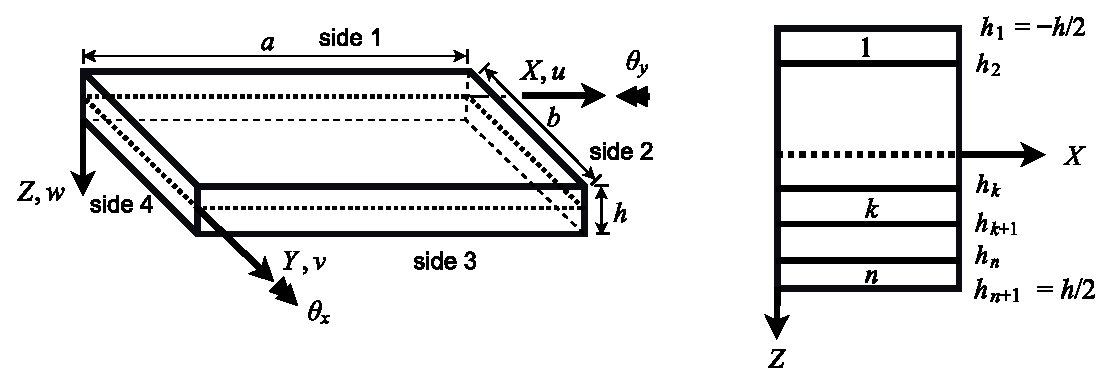
\includegraphics[width=\linewidth]{Laminated_Plate_Final.eps}
	%	\end{minipage}
	\caption{Schematic diagram of a laminated composite plate}
	\label{fig:LaminatedCompositePlate}
\end{figure}

\subsection{Displacement field model}	
For the nonpolynomial shear deformation theory, the plate deformation at any arbitrary point in the plate can be expressed in terms of field variables as

\begin{equation} 	\label{eq:DisplacementModelNPSDT}
\begin{gathered}
u\left(x,y,z\right)=u_{0}\left(x,y\right)-z\frac{\partial w_{0}}{\partial x}+f\left(z\right)\theta_{x}\left(x,y\right)\\
v\left(x,y,z\right)=v_{0}\left(x,y\right)-z\frac{\partial w_{0}}{\partial y}+f\left(z\right)\theta_{y}\left(x,y\right)\\
w\left(x,y,z\right)=w_{0}\left(x,y\right)
\end{gathered}
\end{equation}

where $u_{0}$, $v_{0}$, and $w_{0}$ are the displacements along the mid-plane of the plate; $\theta_{x}$ and $\theta_{y}$ are the shear deformation	at the mid-plane. The function $f\left(z\right) = \left(g\left(z\right)+z\Omega\right)$ incorporate the nonlinearity in transverse strain and represent the warping	of the cross-section perpendicular to mid-plane. For the present study, an inverse hyperbolic shear deformation theory (IHSDT) \cite{grover2013new} is employed by considering $g\left(z\right) = sinh^{-1}\left(\frac{rz}{h}\right)$ and $\Omega = -\frac{2r}{h} \frac{1}{\sqrt{r^{2} + 4}} $ with $r = 3$ in which $h$ is the thickness of the plate.

\subsection{\label{sub:Strain-Displacement-Relation}Strain-displacement relation}
The state-of-strain, $ \boldsymbol{\epsilon} $ at a point corresponding to nonpolynomial displacement fields, in the Cartesian coordinate, is expressed as 
\begin{equation}
%\resizebox{0.5\textwidth}{!}
%{$
\boldsymbol{\epsilon} =\left\{ \begin{array}{c}
\frac{\partial u}{\partial x}\\
\frac{\partial v}{\partial y}\\
\frac{\partial u}{\partial y}+\frac{\partial v}{\partial x}\\
\frac{\partial v}{\partial z}+\frac{\partial w}{\partial y}\\
\frac{\partial u}{\partial z}+\frac{\partial w}{\partial x}
\end{array}\right\} =\left[\begin{array}{ccccc}
\frac{\partial}{\partial x} & 0 & -z\frac{\partial^{2}}{\partial x^{2}} & f\left(z\right)\frac{\partial}{\partial x} & 0\\
0 & \frac{\partial}{\partial y} & -z\frac{\partial^{2}}{\partial y^{2}} & 0 & f\left(z\right)\frac{\partial}{\partial y}\\
\frac{\partial}{\partial y} & \frac{\partial}{\partial x} & -2z\frac{\partial^{2}}{\partial x\partial y} & f\left(z\right)\frac{\partial}{\partial y} & f\left(z\right)\frac{\partial}{\partial x}\\
0 & 0 & 0 & 0 & f^\prime(z)\\
0 & 0 & 0 & f^\prime(z) & 0
\end{array}\right]\left\{ \begin{array}{c}
u_{0}\\
v_{0}\\
w_{0}\\
\theta_{x}\\
\theta_{y}
\end{array}\right\} \label{eq:StrainDisplacementRelation}
%	$}
\end{equation}

The strain vector $ \boldsymbol{\epsilon} $  followed from Eq. \cref{eq:DisplacementModelNPSDT} can be written as summation of in-plane strain vector $\boldsymbol{\epsilon_{p}}=\left\{\epsilon_{xx}\,\,\epsilon_{yy}\,\,\gamma_{xy}\right\}^{T} = \boldsymbol{\epsilon_{p1}} + z \boldsymbol{\epsilon_{p2}} + g(z) \boldsymbol{\epsilon_{p3}}$ and transverse shear strain vector $\boldsymbol{\epsilon_{s}}=\left\{ \gamma_{yz} \,\, \gamma_{xz} \right\}^{T} = \boldsymbol{\epsilon_{s1}} +g'\left(z\right)\boldsymbol{\epsilon_{s2}}$. 

\begin{equation}\label{eq:Strains1}
\boldsymbol{\epsilon}  = 
\left\{
\begin{array}{c}
\boldsymbol{\epsilon_{p}} \\
\boldsymbol{\epsilon_{s}}
\end{array}	
\right\} ,\,\,\,\,
\boldsymbol{\epsilon_{p}}=\left\{ \begin{array}{c}
\frac{\partial u}{\partial x}\\
\frac{\partial v}{\partial y}\\
\frac{\partial u}{\partial y}+\frac{\partial v}{\partial x}
\end{array}\right\} ,\,\,\,\,
\boldsymbol{\epsilon_{s}}=\left\{ \begin{array}{c}
\frac{\partial v}{\partial z}+\frac{\partial w}{\partial y}\\
\frac{\partial u}{\partial z}+\frac{\partial w}{\partial x}
\end{array}\right\}
\end{equation}
where,

\begin{equation}\label{eq:Strains2}
%				\resizebox{0.5\textwidth}{!}
%			{$
\boldsymbol{\epsilon_{p}}=
\left\{ \begin{array}{c}
\frac{\partial u_{o}}{\partial x}\\
\frac{\partial v_{o}}{\partial y}\\
\frac{\partial u_{o}}{\partial y}+\frac{\partial v_{o}}{\partial x}
\end{array}\right\} +z\left\{ \begin{array}{c}
-\frac{\partial^{2}w_{o}}{\partial x^{2}}+\Omega\frac{\partial\theta_{x}}{\partial x}\\
-\frac{\partial^{2}w_{o}}{\partial y^{2}}+\Omega\frac{\partial\theta_{y}}{\partial y}\\
-2\frac{\partial^{2}w_{o}}{\partial x\partial y}+\Omega\left(\frac{\partial\theta_{x}}{\partial y}+\frac{\partial\theta_{y}}{\partial x}\right)
\end{array}\right\} +g(z)\left\{ \begin{array}{c}
\frac{\partial\theta_{x}}{\partial x}\\
\frac{\partial\theta_{y}}{\partial y}\\
\frac{\partial\theta_{x}}{\partial y}+\frac{\partial\theta_{y}}{\partial x}
\end{array}\right\} 
%			$}
\end{equation}

\begin{equation*}
\boldsymbol{\epsilon_{s}}= \Omega \left\{ \begin{array}{c}
\theta_{y}\\
\theta_{x}
\end{array}\right\} +\frac{\partial g}{\partial z}\left\{ \begin{array}{c}
\theta_{y}\\
\theta_{x}
\end{array}\right\} 
\end{equation*}

In Eq. \cref{eq:Strains2}, the presence of second-order derivative operator requires $C^{1}$ continuity of field variable, specifically $w_{0}$. For Navier type analytical solution, $C^{1}$ continuity is easily achieved; however numerical method like FEM, which utilized Lagrange element, gives at most $C^{0}$ continuity of field variables. The reduction of $C^{1}$ to $C^{0}$ continuity requirement in FEM using Lagrange element is achieved by imposing an artificial constraint \cite{grover2014efficient}. So, after incorporating the constraint, the finite element model contains seven field variables. However, IGA can satisfy $C^{1}$ and higher order continuity because of the use of NURBS basis function in it; therefore it utilizes only five field variables \cite{talha2010static}, and as a result no artificial constraints are needed in the strain energy expression.

% as no artificial constraints are needed in the strain energy expression.}

\subsection{Constitutive equation}
The constitutive equation for an arbitrary $k^{th}$ orthotropic layer in global coordinate for plane stress problem is given by the Hooke's law as

\begin{equation}
\boldsymbol{\sigma}^{\left(k\right)}
=\left[\mathcal{T}_{trans}^{\left(k\right)}\right] \boldsymbol{Q} \left[\mathcal{T}_{trans}^{\left(k\right)}\right]^{T}  \boldsymbol{\epsilon}^{\left(k\right)}
=\bar{\boldsymbol{Q}}^{\left(k\right)} \boldsymbol{\epsilon}^{\left(k\right)}\label{eq:ConstitutiveEquation}
\end{equation}

which may be elaborated as

\begin{equation}
%\resizebox{0.5\textwidth}{!}
%{$
\left\{\begin{array}{c}
\sigma_{xx}\\
\sigma_{yy}\\
\sigma_{xy}\\
\sigma_{yz}\\
\sigma_{xz}
\end{array}\right\}^{\left(k\right)}
=
\left[\mathcal{T}_{trans}^{\left(k\right)}\right]
\left[\begin{array}{ccccc}
Q_{11} & Q_{12} & Q_{16} & 0 & 0\\
Q_{21} & Q_{22} & Q_{26} & 0 & 0\\
Q_{61} & Q_{62} & Q_{66} & 0 & 0\\
0 & 0 & 0 & Q_{44} & Q_{45}\\
0 & 0 & 0 & Q_{54} & Q_{55}
\end{array}\right]
\left[\mathcal{T}_{trans}^{\left(k\right)}\right]^{T} 
\left\{\begin{array}{c}
\epsilon_{xx}\\
\epsilon_{yy}\\
\gamma_{xy}\\
\gamma_{yz}\\
\gamma_{xz}
\end{array}\right\}^{\left(k\right)}
%	$}
\end{equation}

where, $ \boldsymbol{\sigma} $, $\boldsymbol{\epsilon} $ and $ \boldsymbol{\bar{Q}} $ are stress vector, strain vector, and the material	constant matrix  in the global coordinate, respectively. And $\left[ \mathcal{T}_{trans} \right]$	is the local-to-global transformation matrix \cite{reddy2004mechanics}. Due to symmetry in the orthotropic material $Q_{21}=Q_{12}$, $Q_{61}=Q_{16}$, $Q_{62}=Q_{26}$, and $Q_{54}=Q_{45}$; each material matrix coefficient can be expressed as
\begin{equation*}
Q_{11}=\frac{E_{1}}{1-\nu_{12}\nu_{21}},\,\,Q_{12}=\frac{\nu_{12}E_{2}}{1-\nu_{12}\nu_{21}},\,\,Q_{22}=\frac{E_{2}}{1-\nu_{12}\nu_{21}}
\end{equation*}
\begin{equation*}
Q_{66}=G_{12},\,\,Q_{44}=G_{23},\,\,Q_{55}=G_{13}
\end{equation*}

Above, $E_{1}$ and $E_{2}$ are the Young's modulus; $G_{12}$, $G_{23}$, and $G_{13}$ are the shear modulus; and $\nu_{12}$ and $\nu_{21}$ are major and minor Poisson's ratios. Where, $1$ represents longitudinal direction, and $2$ and $3$ represent transverse direction.

The in-plane forces, moments and shear forces are defined as
\begin{equation} \label{eq:Resultant}
\begin{gathered}
\left[ \begin{array}{ccc}
\boldsymbol{N} & \boldsymbol{M} & \boldsymbol{P}
\end{array} \right] =
\left[\begin{array}{ccc}
N_{xx} & M_{xx} & P_{xx}\\
N_{yy} & M_{yy} & P_{yy}\\
N_{xy} & M_{xy} & P_{xy}
\end{array}\right]=\int_{-h/2}^{h/2}\left\{ \begin{array}{c}
\sigma_{xx}\\
\sigma_{yy}\\
\sigma_{xy}
\end{array}\right\}
\left\{ \begin{array}{ccc}
1 & z & g\left(z\right)\end{array}\right\}
dz
\\
\left[ \begin{array}{cc}
\boldsymbol{Q} & \boldsymbol{L}
\end{array} \right] =
\left[\begin{array}{cc}
Q_{yz} & L_{yz}\\
Q_{xz} & L_{xz}
\end{array}\right]=\int_{-h/2}^{h/2}\left\{ \begin{array}{c}
\sigma_{yz}\\
\sigma_{xz}
\end{array}\right\} 
\left\{\begin{array}{cc}
1 & g'\left(z\right)\end{array}\right\}
dz
\end{gathered}
\end{equation}

Now, substituting Eq. \cref{eq:ConstitutiveEquation} into Eq. \cref{eq:Resultant}, a generalized stress vector, $\boldsymbol{\hat{\sigma}}$ can be written in term of generalized strain vector, $\boldsymbol{\hat{\epsilon}}$ by following expression

\begin{equation}
\boldsymbol{\hat{\sigma}} =\left\{ \begin{array}{c}
\boldsymbol{N}\\
\boldsymbol{M}\\
\boldsymbol{P}\\
\boldsymbol{Q}\\
\boldsymbol{L}
\end{array}\right\} =\left[\begin{array}{ccccc}
\boldsymbol{A} & \boldsymbol{B} & \boldsymbol{E} & 0 & 0\\
\boldsymbol{B} & \boldsymbol{D} & \boldsymbol{F} & 0 & 0\\
\boldsymbol{E} & \boldsymbol{F} & \boldsymbol{H} & 0 & 0\\
0 & 0 & 0 & \boldsymbol{A}^{s} & \boldsymbol{B}^{s}\\
0 & 0 & 0 & \boldsymbol{B}^{s} & \boldsymbol{D}^{s}
\end{array}\right]\left\{ \begin{array}{c}
\boldsymbol{\epsilon_{p1}}\\
\boldsymbol{\epsilon_{p2}}\\
\boldsymbol{\epsilon_{p3}}\\
\boldsymbol{\epsilon_{s1}}\\
\boldsymbol{\epsilon_{s2}}
\end{array}\right\} = \boldsymbol{\hat{D}} \, \boldsymbol{\hat{\epsilon}} 
\end{equation}

where

\begin{equation*}
\begin{gathered}
\left(\begin{array}{cccccc}
\boldsymbol	A_{ij} & 	\boldsymbol B_{ij}& 	\boldsymbol D_{ij}& 	\boldsymbol E_{ij}&	\boldsymbol F_{ij} & 	\boldsymbol H_{ij} \end{array}\right)
=\int_{-h/2}^{h/2}\left(\begin{array}{cccccc}
1 & z & z^2 & g(z) & zg(z) & g(z)^2 \end{array}\right) \boldsymbol{\bar{Q}_{ij}} \,  dz	\hspace{1cm} i,j\hiderel{=}1,2,6 .
\end{gathered}
\end{equation*}

\begin{equation*}
\begin{gathered}
\left(\begin{array}{ccc}
\boldsymbol{A_{ij}^{s}} & \boldsymbol{B_{ij}^{s}} & \boldsymbol{D_{ij}^{s}}\end{array}\right)=\int_{-h/2}^{h/2}\left(\begin{array}{ccc}
1 & g^{\prime}(z) & g^{\prime}(z)^{2}\end{array}\right) \boldsymbol{\bar{Q}_{ij}} \, dz \hspace{1cm} i,j\hiderel{=}4,5
\end{gathered}
\end{equation*}

\subsection{Equations of motion}
For arbitrary space variable and admissible virtual displacement $\delta\left\{ u\,,v\,,w \right\}$, Hamilton's principle of the given system is written as 

\begin{equation}
%		\resizebox{0.5\textwidth}{!}
%		{$
\delta\int_{t_{i}}^{t_{f}}\mathcal{L}dt=\int_{t_{i}}^{t_{f}}\left(\delta \mathcal{K}-\delta \mathcal{U}+\delta \mathcal{W}_{ext}\right)dt=0
\label{eq:hamilton}
%		$}
\end{equation}%\vspace{0.2cm
The first term in the Eq. \cref{eq:hamilton} represents the virtual kinetic energy and is expressed as

\begin{equation} \label{eq:KineticEnergy}
\delta \mathcal{K} = -\int_{V} \rho \, \delta \boldsymbol{u}^{T} \, \ddot{\boldsymbol{u}} \, dz \, d\Omega
\end{equation}
where $\rho$ is the mass density per unit volume, and $\boldsymbol{u}$ is the displacement vector.
By following Eq. \cref{eq:DisplacementModelNPSDT}, displacement vector, $\boldsymbol{u}$ can be written in matrix form as

\begin{equation} \label{eq:displacementInMatrix}
\boldsymbol{u}  = \boldsymbol{Z} \, \boldsymbol{\bar{u}} 
\end{equation}

which may be elaborated as
\begin{equation*}
\left\{ \begin{array}{c}
u\\
v\\
w
\end{array}\right\} =\left[\begin{array}{ccccccc}
1 & 0 & 0 & f\left(z\right) & 0 & -z & 0\\
0 & 1 & 0 & 0 & f\left(z\right) & 0 & -z\\
0 & 0 & 1 & 0 & 0 & 0 & 0
\end{array}\right]\left\{ \begin{array}{c}
u_{0}\\
v_{0}\\
w_{0}\\
\theta_{x}\\
\theta_{y}\\
w_{0,x}\\
w_{0,y}
\end{array}\right\} 
\end{equation*}

By substituting Eq. \cref{eq:displacementInMatrix} in the Eq. \cref{eq:KineticEnergy} and integrating about Z-direction.  The virtual kinetic energy can be rewritten as

\begin{equation} \label{eq:VirtualKineticEnergy}
\delta \mathcal{K} =
-\int_{\Omega}\delta \boldsymbol{\bar{u}}^{T} \boldsymbol{m} \, \boldsymbol{\ddot{\bar{u}}} \,d\Omega
\end{equation}

where $\boldsymbol{m} $ is the mass matrix, defined by

\begin{equation*}
\boldsymbol{m} = \int^{h/2}_{-h/2} \rho \, \boldsymbol{Z}^{T} \, \boldsymbol{Z} \, dz
\end{equation*}

%	\paragraph*	{\textbf{Strain Energy }}
The second term in the Eq. \cref{eq:hamilton} represents the virtual strain energy and is expressed in terms of generalized stress and strain vector as
%	\begin{equation} 
%	\mathcal{U}=\frac{1}{2}\sum_{k=1}^{n}\int_{\Omega}\left\{ \epsilon^{k}\right\} ^{T}\left\{ \sigma^{k}\right\} d\Omega
%	\end{equation}%\vspace{0.2cm

%	\begin{dmath} 
%		%\begin{equation} 
%		\delta \mathcal{U}=\sum_{k=1}^{n}\int_{\Omega}\delta\left\{ \epsilon^{k}\right\} ^{T}\left\{ \sigma^{k}\right\} d\Omega=\sum_{k=1}^{n}\left(\int_{\Omega}\left(\sigma_{xx}^{k}\delta\epsilon_{xx}^{k}+\sigma_{yy}^{k}\delta\epsilon_{yy}^{k}+\sigma_{xy}^{k}\delta\gamma_{xy}^{k}+\sigma_{yz}^{k}\delta\gamma_{yz}^{k}+\sigma_{xz}^{k}\delta\gamma_{xz}^{k}\right)d\Omega\right)
%		%\end{equation}%\vspace{0.2cm
%	\end{dmath}

\begin{equation} \label{eq:VirtualStrainEnergy}
\delta\mathcal{U}=\int_{\Omega}\delta \boldsymbol{\hat{\epsilon}}^{T}  \boldsymbol{\hat{\sigma}} \, d\Omega=\int_{\Omega}\delta \boldsymbol{\hat{\epsilon}}^T \, \boldsymbol{\hat{D}} \, \boldsymbol{\hat{\epsilon}} \, d \Omega
\end{equation}

%	\begin{equation} 
%	\int_{t_{i}}^{t_{f}}\delta \mathcal{K}dt=-\int_{t_{i}}^{t_{f}}\sum_{k=1}^{n}\left[\int_{\Omega}\delta\left\{ u\right\} \rho^{k}\left\{ \ddot{u}\right\} d\Omega\right]dt
%	\end{equation}%\vspace{0.2cm

%	\paragraph* {\textbf{Work Done }}

The last term of the Eq. \cref{eq:hamilton} is the virtual work done by transverse mechanical load and is expressed as

%	\begin{equation} 
%	%W_{ext}=\int_{A}\left\{ u\right\} ^{T}\left\{ f\right\} dA
%	\mathcal{W}_{ext}=\int_{A} wP dA
%	\end{equation}%\vspace{0.2cm
\begin{equation} \label{eq:VirtualWorkDone}
%\delta W_{ext}=\int_{A}\delta\left\{ u\right\} ^{T}\left\{ f\right\} dA
\delta \mathcal{W}_{ext}=\int_{\Omega}\delta w_{0} P_{w}\left(x, y, t \right) d\Omega
\end{equation}%\vspace{0.2cm
where $P_{w}\left(x, y, t \right)$ is the distributed transverse load.
\section{Isogeometric formulation for composite plate}
\subsection{NURBS functions and surfaces}
After decades of technology improvement, NURBS provides users with great control over the object shape in an intuitive way with low memory consumption making them the most widespread technique for geometry representation \cite{piegl1997monographs,rogers2001introduction}. In this subsection, various fundamental components related to B-spline and NURBS like knot vectors, rational or non-rational basis function are discussed.
\subsubsection{Knot vectors}
%{\color{red}{In FEA the parameter space is the reference element which is mapped into each single element in the physical space. But in IGA, the parameter space consists of several elements (namely knot spans), and the mapping to the physical representation involves all these elements rather than one single [40].}} 
A parametric space is partitioned into elements by a knot vector, $\Xi$ in each direction, which is a non-decreasing set of coordinates in one-dimension \cite{piegl1997monographs,rogers2001introduction}. The knot vector is written as

\begin{equation} \label{eq:KnotVectors}
\Xi=\{\xi_{1},\xi_{2},........,\xi_{j},......,\xi_{n+p+1}\}
\end{equation}

where the length of the knot vector is defined as, $|\Xi|=n+p+1$. Here $\xi_{j}$ denotes the $j^{th}$ knot, $j$ is the knot index, $n$ is the number of basis functions and $p$ is the polynomial degree. In general, there are two main classes of knot vectors namely periodic and open, and the further classification depends on the arrangement of knot values \cite{rogers2001introduction}.

Open knot vectors are standard in the CAD literature. In one-dimension, basis functions formed from open knot vectors are interpolatory at the ends of the parametric space interval, $[\xi_{1},\xi_{n+p+1}]$, but are not interpolatory at the interior knots. This feature makes knots, in isogeometric analysis, different from nodes, in finite element analysis (FEA). An open non-uniform knot vector can be conducive to attain much richer behavior in the characteristics of basis functions used in IGA \cite{cottrell2007studies}.

\subsubsection{Basis functions}
Given a knot vector, the B-spline basis functions, $N_{i,p}^{b}(\xi)$ of degree, $p=0$ are defined as

\begin{equation*}
N^{b}_{i,0}(\xi)=\begin{cases}
1, & \xi_{i}\leq\xi<\xi_{i+1}\\
0, & \text{otherwise}
\end{cases}
\end{equation*}

The basis functions of degree $p>0$ are defined by the following Cox-de Boor recursion formula \cite{piegl1997monographs}. 

\begin{equation}\label{eq:B-spline-N}
N^{b}_{i,p}(\xi)=\frac{\xi-\xi_{i}}{\xi_{i+p}-\xi_{i}}N_{i,p-1}^{b}(\xi)+\frac{\xi_{i+p+1}-\xi}{\xi_{i+p+1}-\xi_{i+1}}N_{i+1,p-1}^{b}(\xi) 
\end{equation}

Which means that basis functions are in parametric form in contrast to FEA, i.e., the Lagrange polynomials are explicit functions. Figure \ref{fig:B-spline basis} illustrates a set of one-dimensional quadratic, cubic, and quartic B-spline basis functions for open uniform knot vectors. A B-spline basis function is $C^{p-1}$ continuous at a single knot. A knot value can appear more than once and is then called a multiple knot. At a knot of multiplicity $\hat{k}$, the continuity is reduced to $C^{p-\hat{k}}$. 

%The B-spline basis (or NURBS) can be enriched by three types of refinements - knot insertion, degree elevation (or order elevation), and degree and continuity elevation. The first two are equivalent to h- and p-refinement respectively, while the last one is k-refinement that does not exist in standard FEM \cite{hughes2005isogeometric}.

\begin{figure}
	\centering
	\begin{minipage}{.45\textwidth}
		\graphicspath{{./All_Images/}}
		\centering
		\includegraphics[width=\linewidth]{Quadratic.eps}
		\subcaption{$\Xi=\{0,0,0,\frac{1}{2},1,1,1\}$} 
	\end{minipage}
	\begin{minipage}{{.45\textwidth}}
		\graphicspath{{./All_Images/}}
		\centering
		\includegraphics[width=\linewidth]{Cubic.eps}
		\subcaption{ $\Xi=\{0,0,0,0,\frac{1}{2},1,1,1,1\}$}
	\end{minipage}\vspace{0.2cm}\\
	\begin{minipage}{{.45\textwidth}}
		\graphicspath{{./All_Images/}}
		\centering
		\includegraphics[width=\linewidth]{Quartic.eps}
		\subcaption{$\Xi=\{0,0,0,0,0,\frac{1}{2},1,1,1,1,1\}$}
	\end{minipage}
	\caption{Illustration of $(a)$ Quadratic,  $(b)$ Cubic and $(c)$ Quartic B-spline basis functions respectively}
	\label{fig:B-spline basis}
\end{figure}

\subsubsection{NURBS surface}

B-spline curves are defined as

\begin{equation}\label{eq:B-spline-C}
C(\xi)=\sum_{i=1}^{n}N^{b}_{i,p}(\xi)\,P_{i}
\end{equation}

where $P_i$ are the control points and $N_{i,p}^{b}(\xi)$ is the $p^{th}$-degree B-spline basis function defined on the open knot vector.

B-spline surfaces are defined by the tensor product of B-spline curves in two parametric dimensions $\xi$ and $\eta$ with two knot vectors, $\Xi=\{\xi_{1},\xi_{2},\,$\ldots.$,\xi_{n+p+1}\}$ and $\mathcal{H}=\{\eta_{1},\eta_{2},\,$\ldots.$,\eta_{m+q+1}\}$ and which is expressed as 

\begin{equation}\label{eq:B-surface}
S(\xi,\eta)=\sum_{i=1}^{n}\sum_{j=1}^{m}N^{b}_{i,p}(\xi)M^{b}_{j,q}(\eta)P_{i,j}
\end{equation}

where $P_{i,j}$ is the bidirectional control net and $N_{i,p}^{b}(\xi)$ and $M_{j,q}^{b}(\eta)$ are the B-spline basis functions defined on the knot vectors $\Xi$ and $\mathcal{H}$ respectively, over an $n \times m$ net of control points, $P_{i,j}$. 

The logical coordinate $(i,\,j)$ of B-spline surface is identically denoted as node \enquote{A} in context of FEM \cite{thai2012static,benson2010isogeometric} and Eq. \cref{eq:B-surface} can be rewritten as

\begin{equation}\label{eq:B-surface-1}
S(\xi,\eta)=\sum_{A=1}^{n\times m}N_{A}^{b}(\xi,\eta)P_{A}
\end{equation}

where $N_{A}^{b}(\xi,\eta)=N^{b}_{i,p}(\xi)\,M^{b}_{j,q}(\eta)$ is the shape function associated with a control point $A$. The superscript $b$ indicates that $N_{A}^{b}$ is a B-spline shape function. 

NURBS curves and surfaces are the generalization of B-splines curves and surfaces. A NURBS entity in $\mathbb{R}^{d}$ Euclidean space is obtained by projecting a B-spline entity in $\mathbb{R}^{d+1}$, where d is the number of physical dimensions. NURBS basis functions are obtained by augmenting every control point, $P_{A}$, in control mesh with the homogeneous coordinate $w_{A}$, which are scalar in nature, also known as weights. Given weights to the control points, make NURBS curves/surfaces rational, which are additional parameters demonstrating the projection from projective geometry. The weighting function is constructed as follow:

\begin{equation}\label{eq:B-surface-2}
w^{g}(\xi,\eta)=\sum_{A=1}^{n\times m}N_{A}^{b}(\xi,\eta)\,w_{A}
\end{equation}

where $w^{g}(\xi,\eta)$ is the common denominator function. The NURBS surfaces are then defined by

\begin{equation}\label{eq:B-surface-3}
S(\xi,\eta)=\frac{\sum_{A=1}^{n\times m}N_{A}^{b}(\xi,\eta)w_{A}P_{A}}{w^{g}(\xi,\eta)}=\sum_{A=1}^{n\times m}R_{A}(\xi,\eta)\,P_{A}
\end{equation}  

where $R_{A}(\xi,\eta)=N_{A}^{b}(\xi,\eta)w_{A}/w^{g}(\xi,\eta)$ is the NURBS basis function.

The choice of the weight in the NURBS basis function depends on the CAD model considered for the analysis and which can be calculated \cite{piegl1997monographs,rogers2001introduction} using Eq. \cref{eq:B-surface-3}. For rectangular geometry, B-spline basis functions are sufficient to represent the geometry accurately by considering $w_{A}^{g} = 1$ \cite{piegl1997monographs,rogers2001introduction}, which is a special case of NURBS basis functions.

The B-spline (or NURBS) can be enriched by three types of refinements - knot insertion, degree elevation (or order elevation), and degree and continuity elevation. The first two are equivalent to h- and p-refinement, respectively, while the last one is k-refinement that does not exist in standard FEM \cite{hughes2005isogeometric}.

\subsection{NURBS based discretization}

Using NURBS basis functions, we interpolate the displacement fields of the plate which can be written as

\begin{equation} \label{eq:DiscretizedDisplacement}
\boldsymbol{u}  = \left\{ \begin{array}{c}
u_{0}\\
v_{0}\\
w_{0}\\
\theta_{x}\\
\theta_{y}
\end{array}\right\} =\sum_{I=1}^{\left(p+1\right)\times\left(q+1\right)}\left[\begin{array}{ccccc}
R_{I} & 0 & 0 & 0 & 0\\
0 & R_{I} & 0 & 0 & 0\\
0 & 0 & R_{I} & 0 & 0\\
0 & 0 & 0 & R_{I} & 0\\
0 & 0 & 0 & 0 & R_{I}
\end{array}\right]\left\{ \begin{array}{c}
u_{0I}\\
v_{0I}\\
w_{0I}\\
\theta_{xI}\\
\theta_{yI}
\end{array}\right\}
\end{equation}

where $\left(p+1\right)\times\left(q+1\right)$ is the number of basis functions and ${R}_{I}\,(\xi,\eta)$ and $\textbf{q}_{I}=\left\{ u_{0I}\,\,v_{0I}\,\,w_{0I}\,\,\theta_{xI}\,\,\theta_{yI} \right\}^{T}$ are the NURBS basis functions and the degrees of freedom associated with control point $I$, respectively.

Substituting Eq. \cref{eq:DiscretizedDisplacement} into Eq. \cref{eq:Strains1}, the generalized strain vector, $ \boldsymbol{\hat{\epsilon}}  $ can be rewritten in terms of elemental displacement vector, $\boldsymbol{q}$ and elemental strain-displacement matrix, $\boldsymbol{B}^{L}$, having degree, $(p,\,q) = 2$

\begin{equation}\label{eq:GeneralizedLinearStrain}
\boldsymbol{\hat{\epsilon}} = \sum_{I=1}^{9} 
\boldsymbol{B}^{L}_{I} \, \boldsymbol{q}_{I}=\boldsymbol{B}^{L} \, \boldsymbol{q}
\end{equation}

in which 
\begin{equation*}
\boldsymbol{B}_{I}^{L}=\left[\begin{array}{ccccc}
\left(\boldsymbol{B}_{I}^{p1}\right)^{T} & \left(\boldsymbol{B}_{I}^{p2}\right)^{T} & \left(\boldsymbol{B}_{I}^{p3}\right)^{T} & \left(\boldsymbol{B}_{I}^{s1}\right)^{T} & \left(\boldsymbol{B}_{I}^{s2}\right)^{T}\end{array}\right]^{T}
\end{equation*}
\begin{equation*}
\boldsymbol{q} = \left\{ 
\begin{array}{ccccccccccc}
u_{01}& v_{01}& w_{01}& \theta_{x1}& \theta_{y1}&  \cdots& u_{09}& v_{09}& w_{09}& \theta_{x9}& \theta_{y9}
\end{array}
\right\}^{T}
\end{equation*}
where $\boldsymbol{B}_I$ is a strain-displacement matrix written in terms of NURBS basis function and its derivatives.

\begin{equation*}
\begin{gathered}
\boldsymbol{B}_{I}^{p1}=\left[\begin{array}{ccccc}
R_{I,x} & 0 & 0 & 0 & 0\\
0 & R_{I,y} & 0 & 0 & 0\\
R_{I,y} & R_{I,x} & 0 & 0 & 0
\end{array}\right]\hspace{1.6cm}
\boldsymbol{B}_{I}^{p2}=\left[\begin{array}{ccccc}
0 & 0 & -R_{I,xx} & \Omega R_{I,x} & 0\\
0 & 0 & -R_{I,yy} & 0 & \Omega R_{I,y}\\
0 & 0 & -2R_{I,xy} & \Omega R_{I,y} & \Omega R_{I,x}
\end{array}\right]
\\
\boldsymbol{B}_{I}^{p3}=\left[\begin{array}{ccccc}
0 & 0 & 0 & R_{I,x} & 0\\
0 & 0 & 0 & 0 & R_{I,y}\\
0 & 0 & 0 & R_{I,y} & R_{I,x}
\end{array}\right]\hspace{1.6cm}
\boldsymbol{B}_{I}^{s1}=\left[\begin{array}{ccccc}
0 & 0 & 0 & 0 & \Omega R_{I}\\
0 & 0 & 0 & \Omega R_{I} & 0
\end{array}\right]
\\
\boldsymbol{B}_{I}^{s2}=\left[\begin{array}{ccccc}
0 & 0 & 0 & 0 & R_{I}\\
0 & 0 & 0 & R_{I} & 0
\end{array}\right]
\end{gathered}
\end{equation*}

The first and second derivatives of NURBS basis functions, used in strain-displacement matrix, can be calculated in terms of B-spline basis functions \cite{hughes2005isogeometric} as shown below:

\begin{equation*}
\frac{\partial R_{i}\left(\xi,\eta\right)}{\partial\xi}=w_{i}\left(\frac{1}{w^{g}}\frac{\partial N_{i}^{b}\left(\xi,\eta\right)}{\partial\xi}-\frac{w_{,\xi}^{g}}{\left(w^{g}\right)^{2}}N_{i}^{b}\left(\xi,\eta\right)\right)
\end{equation*}
\begin{equation*}
\frac{\partial^{2}R_{i}(\xi, \eta)}{\partial\xi^{2}}=w_{i}\left(\frac{1}{w^{g}}\frac{\partial^{2}N_{i}^{b}(\xi,\eta)}{\partial\xi^{2}}-2\frac{w_{,\xi}^{g}}{(w^{g})^{2}}\frac{\partial N_{i}^{b}(\xi,\eta)}{\partial\xi}-\frac{w_{,\xi\xi}^{g}}{(w^{g})^{2}}N_{i}^{b}(\xi,\eta)+2\frac{\left(w_{,\xi}^{g}\right)^{2}}{(w^{g})^{3}}N_{i}^{b}(\xi,\eta)\right)
\end{equation*}
\begin{equation} \label{eq:NURBS_derivative}
\frac{\partial^{2}R_{i}(\xi,\eta)}{\partial\xi \partial\eta}=w_{i}\left(\frac{1}{w^{g}}\frac{\partial^{2}N_{i}^{b}(\xi,\eta)}{\partial\xi\partial\eta}-\frac{w_{,\xi}^{g}}{(w^{g})^{2}}\frac{\partial N(\xi,\eta)}{\partial\eta}-\frac{w_{,\eta}^{g}}{(w^{g})^{2}}\frac{\partial N(\xi,\eta)}{\partial\xi}-\frac{w_{,\xi\eta}^{g}}{(w^{g})^{2}}N_{i}^{b}(\xi,\eta)+2\frac{w_{,\xi}^{g}w_{,\eta}^{g}}{(w^{g})^{3}}N_{i}^{b}(\xi,\eta)\right)
\end{equation}
%	\\\hspace*{-7.5cm}  \text{Where, } \\
%	w^{g}=\sum_{j=1}^{n}w_{j}N_{j}^{b}(\xi),\,\,\,\,\,w_{,\xi}^{g}=\sum_{j=1}^{n}w_{j}\frac{dN_{j}^{b}\left(\xi\right)}{d\xi}
where,

\begin{equation*}
\begin{gathered}
w^{g}=\sum_{j=1}^{n}w_{j}N_{j}^{b}\left(\xi,\eta\right)\hspace{2cm}
w_{,\xi}^{g}=\sum_{j=1}^{n}w_{j}\frac{\partial N_{j}^{b}\left(\xi,\eta\right)}{\partial\xi}\\
w_{,\xi\xi}^{g}=\sum_{j=1}^{n}w_{j}\frac{\partial^{2}N_{j}^{b}\left(\xi,\eta\right)}{\partial\xi^{2}}\hspace{2cm}
w_{,\xi\eta}^{g}=\sum_{j=1}^{n}w_{j}\frac{\partial^{2}N_{j}^{b}\left(\xi,\eta\right)}{\partial\xi\partial\eta}
\end{gathered}
\end{equation*}

To calculate the derivatives of NURBS in Eq. \cref{eq:NURBS_derivative},  $k^{th}$ derivative of B-spline basis function is required and the same can be obtained by following formula \cite{hughes2005isogeometric}

\begin{equation*}
\begin{gathered}
\frac{d^{k}}{d\xi^{k}}N_{i,p}^{b}\left(\xi\right)=\frac{p!}{\left(p-k\right)!}\sum_{j=0}^{k}\beta_{k,j}N_{i+j,p-k}^{b} \left(\xi\right)\\
\begin{aligned}
\beta_{0,\,0}&=1 & k&=0,\,j=0\\
\beta_{k,\,0}&=\frac{\beta_{k-1,\,j}}{\xi_{i+p+j-k+1}-\xi_{i+j}} & j&=0\\
\beta_{k,\,k}&=\frac{-\beta_{k-1,\,j-1}}{\xi_{i+p+j-k+1}-\xi_{i+j}} & j&=k\\
\beta_{k,\,j}&=\frac{\beta_{k-1,\,j}-\beta_{k-1,\,j-1}}{\xi_{i+p+j-k+1}-\xi_{i+j}} & j&=1,\,\cdots,\,k-1
\end{aligned}
\end{gathered}
\end{equation*}

Using  Eqs. \cref{eq:VirtualKineticEnergy,eq:VirtualStrainEnergy,eq:VirtualWorkDone,eq:DiscretizedDisplacement,eq:GeneralizedLinearStrain} in Eq. \cref{eq:hamilton}, and eliminating the virtual displacement vector, $\delta \boldsymbol{q}$, the system of equations of motion for transient analysis (or initial value problem) \cite{krenk2009non} can be obtained in following matrix form
\begin{equation} \label{eq:SystemTransient}
\boldsymbol{K}\boldsymbol{q}+\boldsymbol{M}\boldsymbol{\ddot{q}}=\boldsymbol{F_{m}}
\end{equation}

where $\boldsymbol{K}$, $\boldsymbol{M}$ and $\boldsymbol{F_{m}}$ are the stiffness, mass matrix and force vector, respectively.

\paragraph* {\textbf{Stiffness matrix}}
\begin{equation*}
\boldsymbol{K}=\int\ \boldsymbol{B^{L}}^{T} \,
\boldsymbol{\hat{D}} \, \boldsymbol{B^{L}}  d\Omega
\end{equation*}

\paragraph* {\textbf{Mass matrix}}
\begin{equation*}
\boldsymbol{M} =\int_{\Omega} \left[ \mathcal{R} \right]^{T} \, \boldsymbol{m} \, \left[  \mathcal{R} \right] d\Omega
\end{equation*}
Also, 
\begin{equation*}
\left[  \mathcal{R} \right] \boldsymbol{q} = \sum_{I=1}^{9} \left[  \mathcal{R}_{I} \right] \boldsymbol{q_{I}}
\end{equation*}
where
\begin{equation*}
\left[  \mathcal{R}_{I} \right]=\left[\begin{array}{ccccc}
R_{I} & 0 & 0 & 0 & 0\\
0 & R_{I} & 0 & 0 & 0\\
0 & 0 & R_{I} & 0 & 0\\
0 & 0 & 0 & R_{I} & 0\\
0 & 0 & 0 & 0 & R_{I}\\
0 & 0 & R_{I,x} & 0 & 0\\
0 & 0 & R_{I,y} & 0 & 0
\end{array}\right]
\end{equation*}

\paragraph* {\textbf{Force vector}}
\begin{equation*}
\boldsymbol{F_{m}}=\int_{\Omega} \left\{ \mathcal{W} \right\}^{T}P_{w}\left(x, y, t\right)d\Omega
\end{equation*}

Also,
\begin{equation*}
\left\{ \mathcal{W} \right\} \boldsymbol{q} = \sum_{I=1}^{9} \left\{ \mathcal{W}_{I} \right\} \boldsymbol{q_{I}}
\end{equation*}
where
\begin{equation*}
 \left\{ \mathcal{W}_{I} \right\}=\left\{\begin{array}{ccccc}
0 & 0 & R_{I} & 0 & 0\end{array}\right\}
\end{equation*}

By neglecting the effect of external force in Eq. \cref{eq:SystemTransient}, the governing set of equations for free vibration analysis (or eigenvalue problem) \cite{reddy2004mechanics} is obtained as
\begin{equation*}
\boldsymbol{M}\boldsymbol{\ddot{q}} + \boldsymbol{K}\boldsymbol{q} = 0
\end{equation*}

Similarly, the system of equilibrium equations for static analysis (or boundary value problem) \cite{reddy2004mechanics} is obtained by neglecting the influence of inertial force from Eq. \cref{eq:SystemTransient}  as
\begin{equation*}
\boldsymbol{K} \boldsymbol{q}  = \boldsymbol{F}_{m}
\end{equation*}

\section{Numerical results}
In this section, numerical results of static and dynamic analyses of laminated and sandwich composite plates using NURBS based isogeometric approach in conjunction with NPSDT are presented.

\subsection{Material properties}
Following sets of material properties are used in this section:
\begin{itemize}
	\item Material-I: \cite{reddy2004mechanics}\\
	$
	{E_{1}}/{E_{2}}=25,\,\,\,\,{G_{12}}/{E_2}=0.5,\,\,\,\,{G_{13}}/{E_2}=0.5,\,\,\,\,	{G_{23}}/{E_2}=0.2,\,\,\,\,\nu_{12}=0.25.
	$	
	\item Material-II: \cite{srinivas1973refined}
	
	\begin{equation*}
	\begin{gathered}
	{Q}_{core}=\left[\begin{array}{ccccc}
	0.999781 & 0.231192 & 0 & 0 & 0\\
	0.231192 & 0.524886 & 0 & 0 & 0\\
	0 & 0 & 0.262931 & 0 & 0\\
	0 & 0 & 0 & 0.266810 & 0\\
	0 & 0 & 0 & 0 & 0.159914
	\end{array}\right] \\
	\hspace{-0.9cm}{Q}_{facesheet}=\mathcal{R} \times {Q}_{core};\hspace{1.5cm}\text{where}\,\,\,\,\,\,\,\,\rho_{facesheet}=\mathcal{R} \times \rho_{core}
	\end{gathered}
	\end{equation*}
	
	\item Material-III: \cite{grover2013analytical}\\
	Face sheets:\\
	$
	E_{1}=276\,\,GPa,\,\,\,\,E_{2}=G_{12}=G_{13}=G_{23}=6.9\,\,GPa,\,\,\,\,\nu_{12}=0.25,\,\,\,\,\rho=681.8\,\,kg/m^3.
	$\\
	Core:\\
	$
	E_{1}=E_{2}=0.5776\,\,GPa,\,\,\,\,G_{12}=G_{13}=0.1079\,\,GPa,\,\,\,\,G_{23}=0.22215\,\,GPa,\,\,\,\,\nu_{12}=0.0025,\,\,\,\,\rho=1000\,\,kg/m^3.
	$
	
	\item Material-IV: \cite{kulkarni2008free}\\
	$
	E_{1}=276\,\,GPa,\,\,\,\,E_{2}=6.9\,\,GPa,\,\,\,\,G_{12}=G_{13}=4.14\,\,GPa,\,\,\,\,G_{23}=3.45\,\,GPa,\,\,\,\,\nu_{12}=0.25,\,\,\,\,\rho=1578\,\,kg/m^3.
	$
	\item Material-V: \cite{chen2000nonlinear}\\
	%				\resizebox{0.5\textwidth}{!}{
	$
	E_{1}=525\,\,GPa,\,\,\,\,E_{2}=21\,\,GPa,\,\,\,\,G_{12}=G_{23}=G_{13}=10.5\,\,GPa,\,\,\,\,\nu_{12}=0.25,\,\,\,\,\rho=800\,\,kg/m^3.
	$
	
	\item Material-VI: \cite{tran2015geometrically}\\
	$
	E_{1}=172.369\,\,GPa,\,\,\,\,E_{2}=6.895\,\,GPa,\,\,\,\,G_{12}=G_{13}=3.448\,\,GPa,\,\,\,\,G_{23}=1.379\,\,GPa,\,\,\,\,\nu_{12}=0.25,\,\,\,\,\rho=1603.03\,\,kg/m^3.
	$
	\item Material-VII: \cite{nosier1990effects}\\
	$
	E_{1}=30\times10^6\,\,psi,\,\,\,\,E_{2}=0.75\times10^6\,\,psi,\,\,\,\,G_{12}=0.45\times10^6\,\,psi,\,\,\,\,G_{23}=G_{13}=0.37\times10^6\,\,psi,\,\,\,\,\nu_{12}=0.25,\,\,\,\,\rho=0.000143\,\,lb\,sec^2/in^4.
	$		
	%				\item Material-III: (Sandwich) \cite{shariyat2010generalized}\\
	%				Face sheets:\\
	%				$
	%				E_{1}=200\,\,GPa,\,\,\,E_{2}=1\,\,GPa,\,\,\,G_{12}=G_{13}=5\,\,GPa,\\G_{23}=2.2\,\,GPa,\,\,\,\nu_{12}=0.25,\\ \alpha_{1}=-2\times10^{-6}/K,\,\,\,\alpha_{2}=50\times10^{-6}/K.
	%				$\\
	%				Core:\\
	%				$
	%				E_{1}=E_{2}=1\,\,GPa,\,\,\,G_{12}=3.7\,\,GPa,\,\,\,G_{13}=G_{23}=0.8\,\,GPa,\,\,\,
	%				\nu_{12}=0.35,\,\,\,\alpha_{1}=\alpha_{2}=30\times10^{-6}/K.
	%				$
	
	\item Material-VIII: \cite{kulkarni2008free}\\
	$
	E_{1}=181\,\,GPa,\,\,\,\,E_{2}=10.3\,\,GPa,\,\,\,\,G_{12}=G_{13}=7.17\,\,GPa,\,\,\,\,G_{23}=2.87\,\,GPa,\,\,\,\,\nu_{12}=0.28,\,\,\,\,\rho=1578\,\,kg/m^3.
	$
	
	\item Material-IX: \cite{khdeir1988dynamic}\\
	$
	E_{2}=10^{6}\,\,psi,\,\,\,\,E_{1}=40E_{2},\,\,\,\,G_{12}=G_{13}=0.6E_{2},\,\,\,\,G_{23}=0.5E_{2},\,\,\,\,\nu_{12}=0.25,\,\,\,\,\rho=0.00012\,\,lb\,sec^2/in^4.
	$
	
\end{itemize}

\subsection{Various dynamic loads}
The dynamic analysis of laminated and sandwich composite plates under different kinds of time dependent blast pulse load \cite{kazanci2016review} is studied numerically by changing various parameters.	The several form of blast loads are explained here.
\begin{itemize}
	\item Step Loading
	
	For step loading, the expression for the load function can be written as
	\begin{equation} 
	P_{w}(t)=\begin{array}{cc}
	\left\{ \begin{array}{c}
	1,\,\,\,\,\,\,\,\,\,\,\,\,\,\,\,\,\,\,\,\,0\leq t\leq t_{1}\\
	0,\,\,\,\,\,\,\,\,\,\,\,\,\,\,\,\,\,\,\,\,\,\,\,\,\,\,\,\,\,\,\,t\geq t_{1}
	\end{array}\right\}  %& step\,loading
	\end{array}
	\end{equation}
	
	\item Sinusoidal Loading
	
	The sinusoidal pulse can be expressed mathematically as
	\begin{equation} 
	P_{w}(t)=\begin{array}{cc}
	\left\{ \begin{array}{c}
	sin(\pi t/t_{1}),\,\,\,\,0\leq t\leq t_{1})\\
	0,\,\,\,\,t\geq t_{1}
	\end{array}\right\}  %& sine\,loading
	\end{array}
	\end{equation}
	
	\item Explosive Blast Loading
	
	If the explosion occurs at a far distant from the plate, then the blast pressure can be expressed as in terms of the Friedlander exponential decay equations as \cite{gupta1987dynamic}
	
	\begin{equation} 
	P_{w}(t)=\begin{array}{cc}
	\left\{ \begin{array}{c}
	e^{-\Upsilon t},\,\,\,\,\,\,\,\,\,\,\,\,0\leq t\leq t_{1}\\
	0,\,\,\,\,\,\,\,\,\,\,\,\,\,\,\,\,\,\,\,\,\,\,\,t\geq t_{1}
	\end{array}\right\}  %& explosive\,blast\,loading
	\end{array}
	\end{equation}
	
	where, $\Upsilon$ denotes a decay parameter. 
	
	\item Triangular Loading
	
	Sonic boom effect could be modeled as a N-shaped pressure pulse, and such a pulse corresponds to an idealized far-field overpressure produced by any supersonic flying object. The overpressure signature of the N-wave shock pulse can be described by
	
	\begin{equation} 
	P_{w}(t)=\begin{array}{cc}
	\left\{ \begin{array}{c}
	1-t/t_{1},\,\,\,0\leq t\leq rt_{1}\\
	0,\,\,\,t \leq 0\,\,\, \text{and}\,\,\, t \geq rt_{1}
	\end{array}\right\} %& Sonic Boom\,loading
	\end{array}
	\end{equation}
	
	where $r$ denotes the shock pulse length factor. The shape of the pulse depends on $r$. Note that: (i) for $r=1$, N-shaped pulse degenerate into a triangular pulse or triangular blast refers to just a positive impulse; (ii) for $r=2$ a symmetric N-shaped pressure pulse is obtained; while (iii) for $r>2$ the N-shaped pulse becomes an asymmetric impulse.
\end{itemize}
%\item Triangular Loading
%			\begin{equation} 
%			F(t)=\begin{array}{cc}
%			\left\{ \begin{array}{c}
%			1-t/t_{1},\,\,\,0\leq t\leq t_{1}\\
%			0,\,\,\,t\geq t_{1}
%			\end{array}\right\} %& triangular\,loading
%			\end{array}
%			\end{equation}

\subsection{Boundary conditions}

As the present formulation is based on the displacement approach, so it is required to satisfy the kinematics boundary conditions ($u_0$, $v_0$, $w_0$, $\theta_x$, $\theta_y$) only. The different types of boundary conditions, most commonly occurring in practice are considered for isogeometric analysis of laminated and sandwich composite plate to assess the efficacy of the present approach.

\begin{itemize}
	\item Simply supported
	\begin{enumerate}
		\item For cross-ply\\	
		SSSS-1 : $v_0=w_0=\theta_{y}=0$ at $x=0,a$ and $u_0=w_0=\theta_{x}=0$ at $y=0,b$.
		\item For angle-ply\\	
		SSSS-2 : $u_0=w_0=\theta_{y}=0$ at $x=0,a$ and $v_0=w_0=\theta_{x}=0$ at $y=0,b$.
	\end{enumerate}
	\item Clamped
	\begin{enumerate}
		\item CCCC : $u_0=v_0=w_0=\theta_{x}=\theta_{y}=w_{0,x}=w_{0,y}=0$ at $x=0,a$ and $y=0,b$.
	\end{enumerate}
\end{itemize}

\subsection{Numerical examples and discussions }
Present subsection deals with some numerical investigations using NURBS based elements on static, free vibration and transient analysis of composite plates that includes validation and comparison of the present results with the analytical results as well as with the available numerical results. The obtained natural frequency from FFT analysis are validated with the present and available eigenvalue solution. Also, the computational efficacy of isogeometric approach is assessed in reference to the standard finite element approach.

In IGA, each knot span is the physical element, where actual integration is carried out. Also, each control point is associated with the NURBS basis function which makes them shared within the knot spans (elements). A $8 \times 8$ mesh of quadratic NURBS element is used for the present study or otherwise stated. Gauss-Legendre quadrature rule of integration has been employed in all the analysis with selective integration scheme as in FEM \cite{adam2014improved, adam2015improved, prathap2013finite} to avoid shear locking behavior. The order of Gauss points $(p+1)\times(q+1)$ for bending, and $p\times q$ for transverse shear part have been used. Where $p$ and $q$ are the polynomial degrees of the NURBS basis functions in $X$ and $Y$ directions, respectively. The integration is carried out at each element, and the assembly is done at the control points, as IGA uses isoparametric mapping.

%The rectangular plate structure is discretized and the discretization detail of entire plate using mesh-size of $5\times5$ quadratic elements is shown in Figure. \ref{Figure:Discretization}.

The discretization detail of the rectangular plate using mesh-size of $5\times5$ quadratic NURBS elements is shown in Fig. \ref{Figure:Discretization}.  It has been assumed that the thickness and the material for all the layers are the same, otherwise stated.

\begin{figure}
	\graphicspath{{./All_Images/}}
	\centering
	\includegraphics[width=\linewidth]{Control_Mesh}
	\caption{Discretization of rectangular plate using IGA (Control Mesh)}
	\label{Figure:Discretization}
\end{figure}

\begin{flushleft}
	\textbf{Static analysis}
\end{flushleft}
This sub-subsection belongs to the description and discussion of various numerical solved examples for establishing the accuracy, efficiency, and applicability of the proposed isogeometric model using IHSDT for bending analysis. The continuous least square projection (CL2P) procedure \cite{hinton1974local} has been extended from FEA to IGA for stress recovery procedure \cite{hassani2012isogeometrical}. The main idea of using CL2P as a stress recovery technique in IGA are: (i) local extrapolation cannot be performed using basis function used in IGA because interior knots are not interpolatory, hence stresses are achieved on surfaces/contours itself, (ii) alternative to control points, to store the stress contour over whole domain at Gauss points requires a large amount of data space, which can be reduced by getting the stress values at the control point directly, (iii) by directly evaluating the gradient of field variables at the domain there is oscillation in the secondary variables like stresses and the same can be overcome, (iv) stresses now can be treated as a primary variable like displacement and hence accurate representation of stresses are achieved. Hence for the evaluation of stresses in IGA at control points with higher accuracy, CL2P stress recovery technique is used to obtain efficient results.

\subsubsection{Four-layered simply supported square laminated plate}\label{4layaredbending}	
A sinusoidal transverse load ($P_w sin(\pi x/a)sin(\pi y/b)$) is considered for the symmetric cross-ply square ($0^0/90^0/90^0/0^0$) laminated plate. The plate is composed of four orthotropic layers ($Material-I$) of equal thickness and is subjected to simply supported boundary condition. The numerical results for the nondimensional deflection and stresses for various span-to-thickness ratios, $a/h$ are obtained at critical points and are shown in Table \ref{tab:Static_4layer}. The results for deflection and stresses are enumerated with the following nondimensional forms as given below

\[
\bar{w}=w_{0}\left(\frac{a}{2},\,\,\,\frac{b}{2}\right)\left(\frac{100E_{2}h^{3}}{b^{4}P_{w}}\right);
\]

\[
\left[\bar{\sigma}_{xx}\,\,\bar{\,\sigma}_{yy}\,\,\,\bar{\sigma}_{xy}\right]=\left[\sigma_{xx}\,\,\,\sigma_{yy}\,\,\,\sigma_{xy}\right]\left(\frac{h^{2}}{b^{2}P_{w}}\right);
\]

\[
\left[\bar{\sigma}_{yz}\,\,\,\bar{\sigma}_{xz}\right]=\left[\sigma_{yz}\,\,\,\sigma_{xz}\right]\left(\frac{h}{bP_{w}}\right);
\]

{\color{purple}The present formulation is verified with the available results based on various shear deformation theories from the literature \cite{mantari2012new, karama2009new, reddy1984simple, rodrigues2012radial, grover2013new}. It is well known that all mentioned HSDTs neglect the thickness stretching effect (normal deformation $\epsilon_z = 0$), which causes the independent traverse displacement through the plate thickness. So, in order to consider thickness stretching effect, a quasi-3D theory given in literature \cite{tran2018static} has also been considered for the comparison. The present results are found to be in good agreement with 2D as well as quasi-3D HSDTs results as shown in Table \ref{tab:Static_4layer}. Also, the accuracy of the present IGA-IHSDT model with respect to its closed-form solution may be well appreciated. Moreover, the through-thickness distribution of transverse shear stresses based on present IGA model using an inverse hyperbolic distribution are compared and are found to be in good agreement. 

Figure \ref{fig:Static_4layer} shows the variation of normal ($\bar{\sigma}_{xx}$) and transverse shear ($\bar{\sigma}_{yz}$) stresses. It is clear from Fig. \ref{fig:Static_4layer} that the present IGA-IHSDT formulation predicts the transverse shear stresses accurately and can be used to model the laminated plates efficiently.}

\begin{table}
	\caption{\label{tab:Static_4layer}Non-dimensional deflection and stresses for simply supported square laminated $\left(0^{0}/90^{0}/90^{0}/0^{0}\right)$ plate under sinusoidal load}
	\centering{}%
	\resizebox{\columnwidth}{!}{
		\begin{tabular}{llllllll}
			\hline 
			$a/h$ & Source / Model & $\bar{w}(\frac{a}{2},\frac{b}{2})$ & $\bar{\sigma}_{xx}(\frac{a}{2},\frac{b}{2},\frac{h}{2})$ & $\bar{\sigma}_{yy}(\frac{a}{2},\frac{b}{2},\frac{h}{4})$ & $\bar{\sigma}_{xy}(0,0,\frac{h}{2})$ & $\bar{\sigma}_{yz}(\frac{a}{2},0,0)$ & $\bar{\sigma}_{xz}(0,\frac{b}{2},0)$\tabularnewline
			\hline 
			4 & Pagano \cite{pagano1972elastic} & 1.954 & 0.72 & 0.663 & 0.047 & 0.291 & 0.219\tabularnewline
			& Mantari \cite{mantari2012new}& 1.921 & 0.74 & 0.635 & 0.048 & 0.269 & 0.254\tabularnewline
			& Karama \cite{karama2009new} & 1.919 & 0.699 & 0.636 & 0.0459 & 0.226 & 0.226\tabularnewline
			& Reddy \cite{reddy1984simple} & 1.893 & 0.665 & 0.632 & 0.044 & 0.239 & 0.206\tabularnewline
			& Rodrigues \cite{rodrigues2012radial} & 1.8931 & 0.6408 & 0.8506 & 0.0436 & - & 0.216\tabularnewline
			& Quasi-3D \cite{tran2018static}${\dagger}$ & 1.9072 & 0.6535 & 0.6326 & - & 0.2949 & 0.2192\tabularnewline
			& CFS-IHSDT \cite{grover2013new} & 1.9257 & 0.7255 & 0.639 & 0.0473 & 0.27 & 0.25\tabularnewline
			& IGA-IHSDT (Present) & 1.9257 & 0.7240 & 0.6396 & 0.0473 & 0.2699 & 0.2505\tabularnewline
			&  &  &  &  &  &  & \tabularnewline
			10 & Pagano \cite{pagano1972elastic} & 0.743 & 0.559 & 0.401 & 0.028 & 0.196 & 0.301\tabularnewline
			& Mantari \cite{mantari2012new} & 0.73 & 0.561 & 0.395 & 0.028 & 0.176 & 0.3287\tabularnewline
			& Karama \cite{karama2009new} & 0.724 & 0.553 & 0.393 & 0.027 & 0.163 & 0.294\tabularnewline
			& Reddy \cite{reddy1984simple} & 0.715 & 0.546 & 0.389 & 0.027 & 0.153 & 0.264\tabularnewline
			& Rodrigues \cite{rodrigues2012radial} & 0.7227 & 0.546 & 0.4194 & 0.0269 & - & 0.2978\tabularnewline
			& Quasi-3D \cite{tran2018static}${\dagger}$ & 0.7161 & 0.5424 & 0.3877 & - & 0.1903 & 0.3022\tabularnewline
			& CFS-IHSDT \cite{grover2013new} & 0.7284 & 0.5578 & 0.3947 & 0.0275 & 0.176 & 0.3287\tabularnewline
			& IGA-IHSDT (Present) & 0.7284 & 0.5572 & 0.3949 & 0.0274 & 0.1763 & 0.3289\tabularnewline
			&  &  &  &  &  &  & \tabularnewline
			100 & Pagano \cite{pagano1972elastic} & 0.439 & 0.539 & 0.276 & 0.022 & 0.141 & 0.337\tabularnewline
			& Mantari \cite{mantari2012new} & 0.435 & 0.539 & 0.271 & 0.021 & 0.119 & 0.332\tabularnewline
			& Karama \cite{karama2009new} & 0.435 & 0.538 & 0.27 & 0.021 & 0.118 & 0.324\tabularnewline
			& Reddy \cite{reddy1984simple} & 0.434 & 0.538 & 0.27 & 0.021 & 0.112 & 0.29\tabularnewline
			& Rodrigues\cite{rodrigues2012radial} & 0.4303 & 0.5374 & 0.2704 & 0.0212 & - & 0.3352\tabularnewline
			& Quasi-3D \cite{tran2018static}${\dagger}$ & 0.4343 & 0.5368 & 0.2699 & - & 0.1376 & 0.3355\tabularnewline
			& CFS-IHSDT\cite{grover2013new} & 0.4345 & 0.5388 & 0.271 & 0.0214 & 0.1271 & 0.3643\tabularnewline
			& IGA-IHSDT (Present) & 0.4344 & 0.5385 & 0.2710 & 0.0213 & 0.1269 & 0.3643\tabularnewline
			\hline 
			\multicolumn{8}{l}
			{${\dagger}$ Transverse stresses are obtained using equilibrium equations}\tabularnewline
		\end{tabular}
	}
\end{table}

\begin{figure}
	\centering
	\begin{minipage}[c]{\textwidth}
		\graphicspath{{./All_Images/}}
		\centering
		\includegraphics[scale=0.33]{4Layer_Sigma_xx_IGA_NPSDT_Bending_h_By_a_1_10.eps}
	\end{minipage}
	\begin{minipage}{\textwidth}
		\graphicspath{{./All_Images/}}
		\centering
		\includegraphics[scale=0.33]{4Layer_Sigma_yz_IGA_NPSDT_Bending_h_By_a_1_10.eps}
	\end{minipage}
	\text{(E): equilibrium-derived}\\
	\text{(C): constitutively-derived}
	\caption{Variation of stresses, $\bar{\sigma}_{xx}$ and $\bar{\sigma}_{yz}$  across thickness for ($0^0/90^0/90^0/0^0$) laminated plate for $a/h=10$}
	\label{fig:Static_4layer}
\end{figure}

\subsubsection{{\color{purple}Two-layer anti-symmetric square plate}}
{\color{purple} A simply supported laminated ($0^0/90^0$) square plate with $Material-I$ subjected to a sinusoidally distributed transverse load is considered.  The numerical results for the nondimensional central deflection with various span-to-thickness ratios, $a/h$ ranging from $5$ to $100$ are obtained using nondimensional forms given in \cref{4layaredbending}. For this example, the present IGA-IHSDT results are compared with the solutions obtained from 3D elasticity \cite{pagano1970exact}, analytical \cite{kant2002analytical} and other numerical approach \cite{tran2014isogeometric,SSarangan2017} which are shown in Table \ref{tab:Static_2layer}. Here this example is specifically considered to show the comparison between the present five variables results with other advanced HSDTs with only four variables. It can be seen from the Table \ref{tab:Static_2layer} that the results using present IGA-IHSDT model are in well agreement with other available four and five variables HSDTs, and zigzag model.}

\begin{table}
	\caption{\label{tab:Static_2layer}Non-dimensional central deflection, $\bar{w}$ for simply supported square laminated $\left(0^{0}/90^{0}\right)$ plate under sinusoidally distributed load with various $a/h$ ratios}
\begin{centering}
		\begin{tabular}{lllll}
			\hline 
			Source / Method & \multicolumn{4}{c}{$a/h$}\tabularnewline
			\cline{2-5} 
			& 5 & 10 & 20 & 100\tabularnewline
			\hline 
			Pagano \cite{pagano1970exact} & 1.7287 & 1.2318 & 1.1060 & 1.0742\tabularnewline
			Reddy \cite{kant2002analytical}{**} & 1.6670 & 1.2161 & 1.1018 & 1.0651\tabularnewline
			Senthilnathan et al. \cite{kant2002analytical}{*} & 1.6670 & 1.2161 & 1.1018 & 1.0651\tabularnewline
			Karama \cite{tran2014isogeometric}{*} & 1.6382 & 1.2096 & 1.1002 & 1.0650\tabularnewline
			IZT-FEM \cite{SSarangan2017}${\dagger}$ & 1.6449 & 1.2087 & - & -\tabularnewline
			IGA-IHSDT (Present){**} & 1.6009 & 1.2009 & 1.0981 & 1.0650\tabularnewline
			\hline 
			\multicolumn{5}{l}
			{${\dagger}$ IZT-FEM - Inverse hyperbolic zigzag theory}\tabularnewline
			\multicolumn{5}{l}
			{${*}$ Four variable HSDT}\tabularnewline
			\multicolumn{5}{l}
			{${**}$ Five variable HSDT}\tabularnewline
		\end{tabular}
		\par\end{centering}
\end{table}

\subsubsection{Three-layered simply supported square sandwich plate}	
A simply supported square sandwich plate ($0^0/C/0^0$) with equal thickness ($h_f=0.1h$) face sheets as shown in Fig. \ref{fig:Sandwich} with orthotropic core composed of material model given in $Material-II$ is analyzed under the effect of uniform load.

\begin{figure}
	\graphicspath{{./All_Images/}}
	\centering
	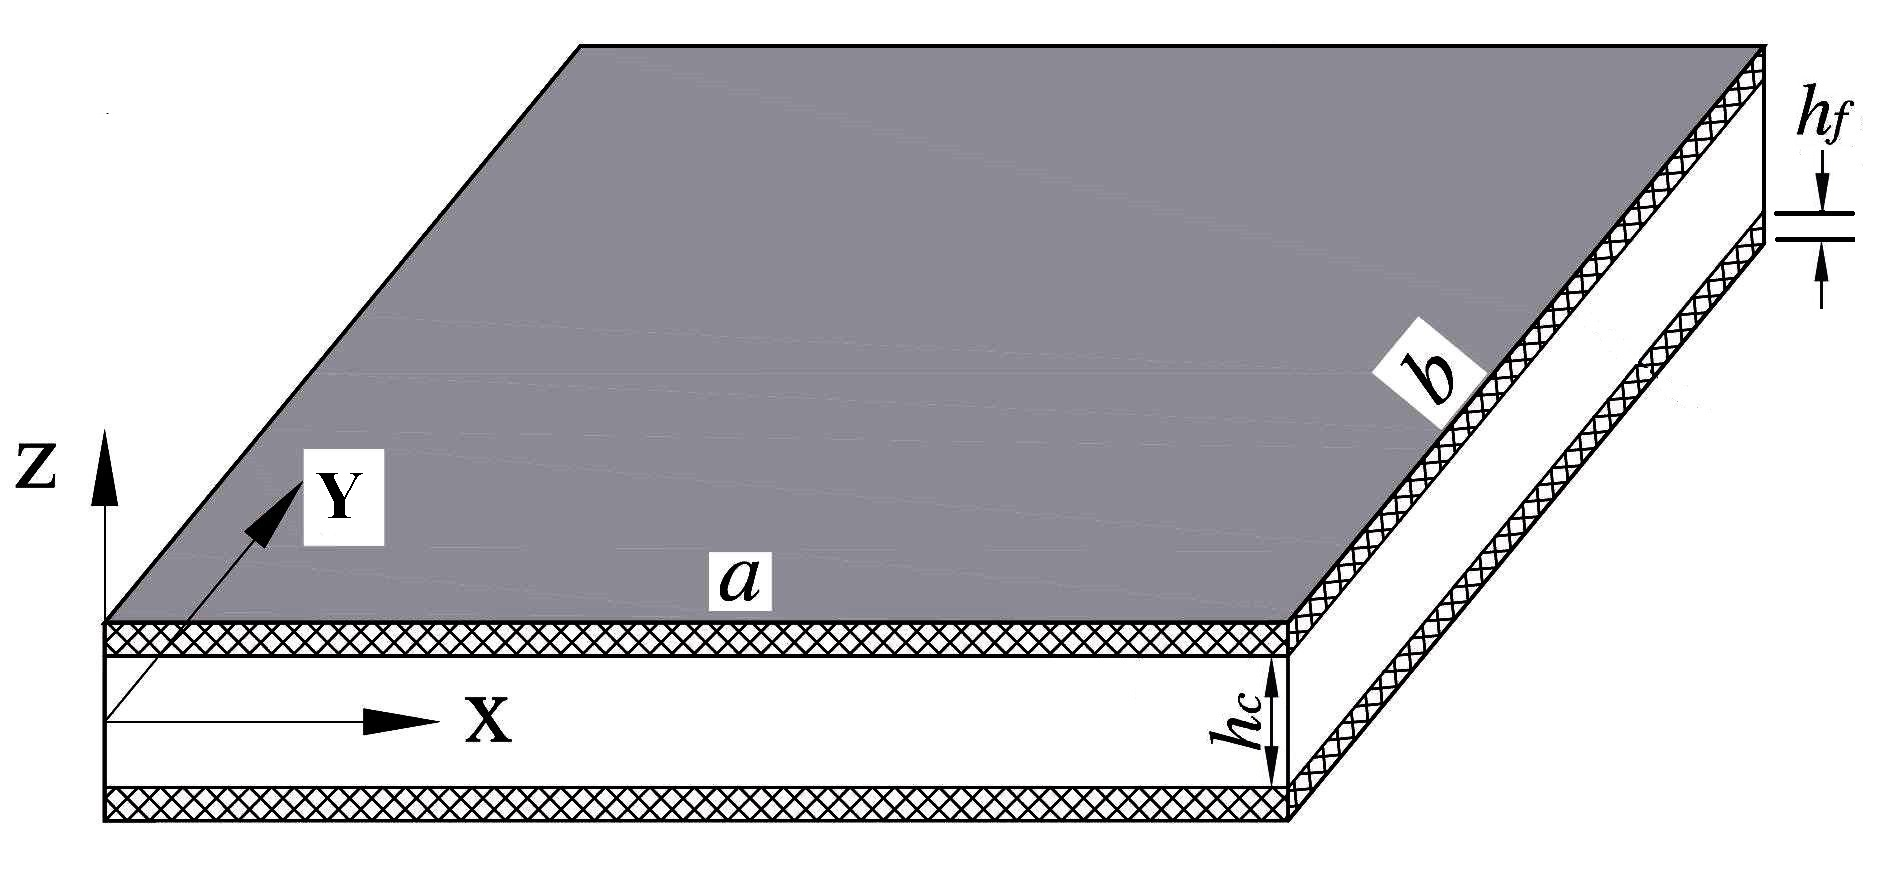
\includegraphics[scale=0.23]{sandwichplate}
	\caption{Schematic diagram of a sandwich plate with face sheets and core}%\vspace*{-6pt}
	\label{fig:Sandwich}
\end{figure}

The material properties of the face sheets are obtained by multiplying core properties by a parameter $\mathcal{R}$. Flexural response of a moderately thick plate is investigated for $\mathcal{R}$ = 5 and 15. Transverse deflection and stresses are obtained at the critical points and the results are presented in the nondimensional forms as given below
% Preview source code from paragraph 9 to 12

\[
\bar{w}=\frac{0.999781}{hP_{w}}\left(\frac{a}{2},\,\,\,\frac{b}{2},\,\,\,0\right);\,\,\,\,\,\,\,\,\,\,\,\,\bar{\sigma}_{xx}^{1}=\frac{\sigma_{xx}^{1}}{P_{w}}\left(\frac{a}{2},\,\,\,\frac{b}{2},\,\,\,-\frac{h}{2}\right);
\]

\[
\bar{\sigma}_{xx}^{2}=\frac{\sigma_{xx}^{1}}{P_{w}}\left(\frac{a}{2},\,\,\,\frac{b}{2},\,\,\,-\frac{2h}{5}\right);\,\,\,\,\,\,\,\,\,\,\,\,\bar{\sigma}_{xx}^{3}=\frac{\sigma_{xx}^{2}}{P_{w}}\left(\frac{a}{2},\,\,\,\frac{b}{2},\,\,\,-\frac{2h}{5}\right);
\]

\[
\bar{\sigma}_{yy}^{1}=\frac{\sigma_{yy}^{1}}{P_{w}}\left(\frac{a}{2},\,\,\,\frac{b}{2},\,\,\,-\frac{h}{2}\right);\,\,\,\,\,\,\,\,\,\,\,\,\bar{\sigma}_{yy}^{2}=\frac{\sigma_{yy}^{1}}{P_{w}}\left(\frac{a}{2},\,\,\,\frac{b}{2},\,\,\,-\frac{2h}{5}\right);
\]

\[
\bar{\sigma}_{yy}^{3}=\frac{\sigma_{yy}^{2}}{P_{w}}\left(\frac{a}{2},\,\,\,\frac{b}{2},\,\,\,-\frac{2h}{5}\right);
\]

In the above expression, superscript over the stresses, i.e., $\sigma_{ii}$ denotes the layer number of the sandwich plate. Numerical results obtained from the present IGA-IHSDT analysis are validated with the existing numerical results based on different shear deformation theories \cite{xiang2009analysis, ferreira2003analysis, mantari2012new, grover2014efficient, grover2013new} and with the closed-form solution (CFS) \cite{srinivas1973refined}. The results are presented in Table \ref{tab:Static_sandwich}. It is observed that IGA results using IHSDT are not only in excellent agreement with the existing results but IGA-IHSDT results are more close to closed-form results than FEM-IHSDT results because of $C^1$-continuity.

\begin{table}
	\caption{\label{tab:Static_sandwich}Static behavior of simply supported sandwich plate $(0^0/C/0^0)$ subjected to uniform load}
	\centering{}%
	\resizebox{\columnwidth}{!}{
		\begin{tabular}{lllllllll}
			\hline 
			$\mathcal{R}$ & Source / Model & $\bar{w}$ & $\bar{\sigma}_{xx}^{1}$ & $\bar{\sigma}_{xx}^{2}$ & $\bar{\sigma}_{xx}^{3}$ & $\bar{\sigma}_{yy}^{1}$ & $\bar{\sigma}_{yy}^{2}$ & $\bar{\sigma}_{yy}^{3}$\tabularnewline
			\hline 
			\multirow{9}{*}{5} & Pagano \cite{srinivas1973refined} & 258.97 & 60.353 & 46.623 & 9.34 & 38.491 & 30.097 & 6.161\tabularnewline
			& Pandya and Kant \cite{pandya1988higher} & 258.74 & 62.38 & 46.91 & 9.382 & 38.93 & 30.33 & 6.065\tabularnewline
			& Touratier \cite{xiang2009analysis}{$\dagger$} & 253.989 & 60.123 & 47.097 & 9.419 & 38.249 & 30.187 & 6.037\tabularnewline
			& Karama \cite{xiang2009analysis}{$\dagger$} & 253.638 & 60.124 & 46.703 & 9.34 & 38.242 & 30.02 & 6.004\tabularnewline
			& Ferreira et al. \cite{ferreira2003analysis} & 257.11 & 60.366 & 47.003 & 9.401 & 38.456 & 30.242 & 6.048\tabularnewline
			& Mantari et al. \cite{mantari2012new}& 256.706 & 60.525 & 47.061 & 9.412 & 38.452 & 30.177 & 6.035\tabularnewline
			& FEM-IHSDT \cite{grover2014efficient} & 255.28 & 59.7731 & 46.5043 & 9.3008 & 38.0231 & 29.8858 & 5.9772\tabularnewline
			& CFS-IHSDT \cite{grover2013new} & 255.644 & 60.6752 & 47.055 & 9.4109 & 38.5223 & 30.2056 & 6.0411\tabularnewline
			& IGA-IHSDT (Present) & 255.623 & 60.55 & 47.033 & 9.4066 & 38.447 & 30.189 & 6.0377\tabularnewline
			&  &  &  &  &  &  &  & \tabularnewline
			\multirow{9}{*}{15} & Pagano \cite{srinivas1973refined}& 121.72 & 66.787 & 48.299 & 3.232 & 46.424 & 34.955 & 2.494\tabularnewline
			& Pandya and Kant \cite{pandya1988higher}& 110.43 & 66.62 & 51.97 & 3.465 & 44.92 & 35.41 & 2.361\tabularnewline
			& Touratier \cite{xiang2009analysis}{$\dagger$} & 113.964 & 66.544 & 50.679 & 3.378 & 45.431 & 35.278 & 2.351\tabularnewline
			& Karama \cite{xiang2009analysis}{$\dagger$} & 114.585 & 66.621 & 49.663 & 3.31 & 45.546 & 34.919 & 2.327\tabularnewline
			& Ferreira et al. \cite{ferreira2003analysis}& 114.644 & 66.92 & 50.323 & 3.355 & 45.623 & 35.17 & 2.345\tabularnewline
			& Mantari et al. \cite{mantari2012new}& 115.919 & 67.185 & 49.769 & 3.318 & 45.91 & 35.081 & 2.339\tabularnewline
			& FEM-IHSDT \cite{grover2014efficient}& 115.83 & 66.4816 & 49.1148 & 3.2743 & 45.4806 & 34.6972 & 2.3131\tabularnewline
			& CFS-IHSDT \cite{grover2013new}& 115.82 & 67.2717 & 49.8129 & 3.3209 & 45.9669 & 35.088 & 2.3392\tabularnewline
			& IGA-IHSDT (Present) & 115.811 & 67.08 & 49.849 & 3.3232 & 45.85 & 35.103 & 2.3402\tabularnewline
			\hline
			\multicolumn{8}{l}
			{${\dagger}$ Xiang et al. \cite{xiang2009analysis}}
		\end{tabular}
	}
\end{table}

\begin{flushleft}
	\textbf{Free Vibration analysis}
\end{flushleft}
Numerous examples are solved to ensure the validity and accuracy of IGA-IHSDT solution for the prediction of eigenvalue. Fundamental natural frequency is obtained and the comparison is made with the existing results.% Different materials are considered and the plates include orthotropic, laminated and sandwich plates.

%{\color{red}	\subsubsection{Four-layer simply supported square laminated plate}
%A four-layer ($0^0/90^0/90^0/0^0$) simply supported symmetric cross-ply square laminated plate is considered to determine the free vibration characteristic. Each cross-ply consist of orthotropic material, $Material-III$, with equal thickness. The effect of the span-to-thickness ratio, $a/h$ on the nondimensional frequency parameter is observed using the IGA-IHSDT and compared with the available closed-form \cite{kulkarni2008free, grover2013new} as well as 3-Dimensional solutions \cite{kulkarni2008free}. A comparison of the present result for different $a/h$ $(5,\,10,\,20)$ ratios is shown in Table \ref{tab:Free_Vib_Laminated1}. It is clear from the table that the present formulation gives very close results to the closed-form result \cite{grover2013new}.}
%
%\begin{table}[htb]
%	\caption{\label{tab:Free_Vib_Laminated1}A non-dimensional frequency parameter $\bar{\omega}=(\omega a^{2}/h)(\rho/E_{2})^{1/2}$	of a $\left(0^{0}/90^{0}/90^{0}/0^{0}\right)$ simply supported laminated	square plate at various $a/h$. }
%	\centering{}%
%	\begin{tabular}{cccc}
%		\hline 
%		Source / Model &  & \multicolumn{2}{c}{$a/h$}\tabularnewline
%		\cline{2-4} 
%		& 5 & 10 & 20\tabularnewline
%		\hline 
%		3-Dimensional \cite{kulkarni2008free}& 8.5611 & 11.2981 & 12.721\tabularnewline
%		CFS-TOT \cite{kulkarni2008free} & 8.7167 & 11.424 & 12.771\tabularnewline
%		CFS-SDTSF \cite{grover2013new} & 8.7170 & 11.4243 & 12.7711\tabularnewline
%		CFS-ITSDT \cite{grover2013new} & 8.6241 & 11.3507 & 12.7424\tabularnewline
%		CFS-IHSDT \cite{grover2013new} & 8.6216 & 11.3481 & 12.7413\tabularnewline
%		IGA-IHSDT (Present) & 8.62155 & 11.348 & 12.7413\tabularnewline
%		\hline 
%	\end{tabular}
%\end{table}
\subsubsection{Five-layered simply supported square sandwich plate}
A five-layered simply supported sandwich plate with symmetric face sheets $(0^{0}/90^{0}/C/90^{0}/0^{0})$ is considered for the analysis. The material properties of core and face sheets are taken from $Material-III$. The ratio of core thickness to the total thickness $h_c/h$ is considered as $0.8$ and the plies of face sheets are assumed to be  of same thickness. The effect of the various span-to-thickness ratios,  $a/h$ $(6.67,\,10,\,20)$ on the nondimensional frequency parameter is observed using IGA-IHSDT and compared with the available solutions as shown in Table \ref{tab:Free_Vib_Sandwich}. The present theory is capable of predicting free vibration behavior of sandwich plates accurately. The results obtained using IGA-IHSDT formulation for sandwich  plate are found to be closer to the analytical results \cite{grover2013analytical} as compared with the other available results. Thus the present formulation has been validated for the free vibration analysis. %{\color{blue}Hence the accuracy of present method may be appreciated.}


\begin{table}
	\caption{\label{tab:Free_Vib_Sandwich}A non-dimensional natural frequency parameter $\bar{\omega}=(100\omega a)(\rho_{c}/E_{1f})^{1/2}$	of a $\left(0^{0}/90^{0}/C/90^{0}/0^{0}\right)$ simply supported	square sandwich plate with $h_{c}/h=0.8$}
	\centering{}%
	\begin{tabular}{llll}
		\hline 
		Source / Model &   \multicolumn{3}{c}{$a/h$}\tabularnewline
		\cline{2-4} 
		& 6.67 & 10 & 20\tabularnewline
		\hline 
		3-Dimensional \cite{kulkarni2008free} & 10.5235 & 9.8281 & 7.6882\tabularnewline
		Wang \cite{wang2000free} & 11.414 & 10.555 & 8.029\tabularnewline
		FEM-TOT \cite{kulkarni2008free} & 13.315 & 12.088 & 8.721\tabularnewline
		CFS-IHSDT \cite{grover2013analytical}& 12.1389 & 11.1572 & 8.3258\tabularnewline
		IGA-IHSDT (Present) & 12.1395 & 11.1575 & 8.3259\tabularnewline
		\hline 
	\end{tabular}
\end{table}

\subsubsection{Higher modes of vibration for simply supported anti-symmetric cross-ply laminated plate}
In order to verify the accuracy for the prediction of higher vibration modes which is used in modal decomposition analysis, a study is conducted on anti-symmetric cross-ply laminated plate. A four-layered $\left(0^{0}/90^{0}/0^{0}/90^{0}\right)$ square laminated plate with span-to-thickness ratio, $a/h=10$ is considered. Material properties used for the analysis is $Material-IV$ for each cross-ply with all edges simply supported. Nondimensional frequencies for first six modes are obtained using present IGA-IHSDT; and a closed form solution (CFS) is also obtained for comparison using method prescribed in the literature \cite{grover2013analytical}.  A comparison of present results with those available in literature are shown in Table \ref{tab:Free_Vib_antisymmetric}. It is observed from the table that the present IGA-IHSDT formulation is also capable of accurately predicting the higher vibration mode of a system and results are in well agreement to closed-form solution.     

\begin{table}
	\caption{\label{tab:Free_Vib_antisymmetric}First six natural frequencies of anti-symmetric laminated plate $\left(0^{0}/90^{0}/0^{0}/90^{0}\right)$ under simply supported boundary condition with $a/h=10$}
	\centering{}%
	\resizebox{\columnwidth}{!}{
		\begin{tabular}{lllllll}
			\hline 
			Mode & CFS-IHSDT${*}$  & IGA-IHSDT (Present) & FEM-IHSDT \cite{grover2013analytical} & 3D \cite{kulkarni2008free} & ZZ \cite{kulkarni2008free} & ZZ \cite{chakrabarti2004vibration} \tabularnewline
			\hline 
			1 & 14.8390 & 14.8390 & 14.8302 & 14.7668 & 14.754 & 14.712\tabularnewline
			2 & 33.1887 & 33.1901 & 33.1266 & 32.7998 & 32.772 & 32.178\tabularnewline
			3 & 33.1887 & 33.1901 & 33.1266 & 32.7998 & 32.772 & 32.178\tabularnewline
			4 & 44.7320 & 44.7341 & 44.6260 & 44.1645 & 44.011 & 42.651\tabularnewline
			5 & 55.6689 & 55.6916 & 55.4164 & 54.5818 & 54.571 & 51.827\tabularnewline
			6 & 55.6689 & 55.6916 & 55.4164 & 54.818 & 54.571 & 51.827\tabularnewline
			\hline 
			\multicolumn{6}{l}
			{${*}$ Results obtained using method prescribed in the literature \cite{grover2013analytical}}\tabularnewline
		\end{tabular}
	}
\end{table}
\begin{flushleft}
	\textbf{Transient analysis}
\end{flushleft}
Time-dependent transient equations are solved using the unconditionally stable Newmark time integration scheme \cite{krenk2009non}. The values of $\alpha$ and $\beta$ are taken to be $0.5$ and $0.25$ (constant-average acceleration method) respectively or otherwise stated.

\subsubsection{Simply supported orthotropic plate under uniform step loading}
In order to  validate the present technique, an orthotropic simply supported plate under uniformly distributed transverse load has been considered. The square plate with length, $a=0.25\,m$ is analyzed using $Material-V$ for the span-to-thickness ratio, $a/h=50$.

An uniform step loading of $1 MPa$ is applied and response is taken at every time step of $\Delta t=10^{-5}\,sec$ for $t_{1}=2 \times 10^{-3}\,sec$ as followed in the reference \cite{chen2000nonlinear}. A transient response  of a nondimensionalized central deflection, $\bar{w}=w/h$ is shown in Fig. \ref{fig:TransientOrtho}. It is observed that the results obtained from IGA-IHSDT are well match with the available finite strip method (FSM) by Chen et. al \cite{chen2000nonlinear} and IGA-TSDT by Tran et. al \cite{tran2015geometrically}. Thus the present formulation has been validated accurately.

\begin{figure}
	\graphicspath{{./All_Images/}}
	\centering
	\includegraphics[scale=0.3]{IGA_NPSDT_Transient_h_By_a_1_50.eps}
	\caption{\label{fig:TransientOrtho}Time history response of the transverse displacement of an orthotropic plate under step loading with spatial uniform distributed load of intensity $1 MPa$}
\end{figure}

Also, to assess the computational efficacy, the variation of total computational time with respect to total number of elements for both FEA and IGA is studied as shown in  Fig. \ref{fig:computational_efficiency_transient}. The comparative study reveals that the IGA requires less computation power than FEA. As the total number of elements increases, the total simulation time of FEA increases drastically, whereas IGA computational time grows gradually, because for the same mesh size IGA requires less control points/ DOFs than FEA and hence IGA solution time is highly reduced. This important aspect of IGA has a far reaching impact on the complex real world problem over FEM where large number of elements are required.
\begin{figure}
	\graphicspath{{./All_Images/}}
	\centering
	\includegraphics[scale=0.5]{Computational_Efficiency_Transient_IGA_FEM.eps}
	\caption{\label{fig:computational_efficiency_transient}The total simulation time plotted against the total number of elements for an orthotropic plate under step loading with spatial uniformly distributed load of intensity $1 MPa$ under transient analysis}
\end{figure}

\subsubsection{Effect of various dynamic loadings on symmetric cross-ply laminated plate}
The dynamic response of three-layered ($0^0/90^0/0^0$) thick laminated plate is investigated using $Material-VI$ for the simply supported boundary condition. Sinusoidally distributed transverse load of magnitude $0.689\,\,GPa$ is used for the analysis of laminated plate with $a/h=5$ and $h=0.1526\,\,m$. Different time dependent impulse loadings: step, triangular, sinusoidal and explosive blast loading are considered for the analysis and results are shown in Fig. \ref{fig:Transient_Tran}. 

The response of nondimensionalized central deflection, $\bar{w}=w/h$ is taken at every time step of $\Delta t=10^{-5} sec$ for $t_{1}=6 \times 10^{-3} sec$. The decay parameter, $\Upsilon$ considered in explosive blast loading is $660 \text{ } sec^{-1}$ as followed in the reference \cite{tran2015geometrically}. Figure \ref{fig:Transient_Tran} shows the comparison of present results with the available result in the literature \cite{tran2015geometrically}, which are found to be in good agreement.

\begin{figure}
	\centering
	\begin{minipage}{0.515\textwidth}
		\graphicspath{{./All_Images/}}
		\centering
		\includegraphics[width=\linewidth]{Tran_Step_NPSDT_Transient_h_By_a_1_5.eps}\\
		\subcaption{\centering Step Loading}
	\end{minipage}\\
	\begin{minipage}{0.515\textwidth}
		\graphicspath{{./All_Images/}}
		\centering
		\includegraphics[width=\linewidth]{Tran_Tri_NPSDT_Transient_h_By_a_1_5.eps}\\
		\subcaption{\centering Triangular Loading}
	\end{minipage}\\
	\begin{minipage}{0.515\textwidth}
		\graphicspath{{./All_Images/}}
		\centering
		\includegraphics[width=\linewidth]{Tran_Sin_NPSDT_Transient_h_By_a_1_5.eps}\\
		\subcaption{\centering Sinusoidal Loading}
	\end{minipage}\\
	\begin{minipage}{0.515\textwidth}
		\graphicspath{{./All_Images/}}
		\centering
		\includegraphics[width=\linewidth]{Tran_Exp_NPSDT_Transient_h_By_a_1_5.eps}\\
		\subcaption{\centering Explosive Loading}
	\end{minipage}
	\caption{Effect of various dynamic loads on the deflection of the cross-ply ($0^0/90^0/0^0$) square laminated plate}
	\label{fig:Transient_Tran}
\end{figure}

\subsubsection{Three-layered square sandwich plate under step loading}
A simply supported square sandwich plate with core thickness, $0.8h$ and face thickness $0.1h$ under sinusoidal and uniform transverse load is considered. The material properties of the sandwich core and skin are given in $Material-II$, where $\rho_{core}=1$. The skins material properties are related with the core properties by $\mathcal{R}$ = 15. Isogeometric square sandwich composite plates with span-to-thickness ratio, $a/h = 10$  subjected to step loading is considered. For this case of sandwich plate, time step for Newmark's direct integration method \cite{roque2011transient} is $\Delta t=10^{-2} sec$ where the values of $\alpha$ and $\beta$ are taken to be $3/2$ and $8/5$  with total simulation time, $t_{1}=25\,sec$ \cite{roque2011transient}.

The plotting of central deflection, $w$ with time $t$ is shown in Fig. \ref{fig:Transient_Sandwich}. It has been observed that the IGA-IHSDT results are in good agreement with the available analytical \cite{roque2011transient}  and FEM-TSDT \cite{roque2011transient} results.

\begin{figure}
	\centering
	\begin{minipage}{\textwidth}
		\graphicspath{{./All_Images./}}
		\centering
		{\includegraphics[scale=0.3]{Step_SSL_Sandwich_IGA_NPSDT_Transient_h_By_a_1_10.eps}}
		\subcaption{Sinusoidal Distribution of Load}
	\end{minipage}\vspace{0.5cm}
	\begin{minipage}{\textwidth}
		\graphicspath{{./All_Images./}}
		\centering
		{\includegraphics[scale=0.3]{Step_UDL_Sandwich_IGA_NPSDT_Transient_h_By_a_1_10.eps}}
		\subcaption{Uniform Distribution of Load}
	\end{minipage}
	\caption{Sandwich plate under step loading}
	\label{fig:Transient_Sandwich}
\end{figure}

\subsubsection{Nine-layered square laminated plate under N-shaped pressure pulse}
The dynamic response of nine-layered $(0^0/90^0/0^0)_3$ simply supported laminated plate is investigated using $Material-VII$. Uniformly distributed transverse load of magnitude $200\,psi$ is used for the analysis with $a/h=20$ and $h=3 \,\,in$. The present analysis consider a symmetric and asymmetric N-shaped pressure pulse with $r=2$ and $2.5$ for $t_{1}=0.01\,sec$ and $0.004\,sec$ respectively as given in the literature \cite{nosier1990effects}. Figure \ref{fig:Transient_triangular} displays the time-history response of dimensionless central deflection ( $\bar{w}=w/h$) obtained for various pulse loads characterized by different $r$ and $t_1$ parameters. It can be seen from the Fig. \ref{fig:Transient_triangular} that the present IGA-IHSDT results are in well agreement with the available results \cite{nosier1990effects}. Hence, it may be concluded that the present IGA-IHSDT formulation is efficient for the transient analysis.

\begin{figure}
	\centering
	\begin{minipage}{\textwidth}
		\graphicspath{{./All_Images./}}
		\centering
		{\includegraphics[scale=0.3]{Structure_b_2_Tri_IGA_NPSDT_Transient_h_By_a_1_20.eps}}
		\subcaption{r=2 and $t_1=0.01 sec$}
	\end{minipage}\vspace{0.5cm}
	\begin{minipage}{\textwidth}
		\graphicspath{{./All_Images./}}
		\centering
		{\includegraphics[scale=0.3]{Structure_b_2_5_Tri_IGA_NPSDT_Transient_h_By_a_1_20.eps}}
		\subcaption{r=2.5 and $t_1=0.004 sec$}
	\end{minipage}
	\caption{Time-history of the nondimensional	central deflection of laminated composite plates to an asymmetric N-shaped pressure pulse}
	\label{fig:Transient_triangular}
\end{figure}

\subsubsection{Time-history response and its Fourier transform for the square laminated plate}
A four-layered ($0^0/90^0/90^0/0^0$) simply supported symmetric cross-ply square laminated plate is considered to determine the nondimensional natural frequency. Each cross-ply consists of orthotropic material, $Material-VIII$, with equal thickness. The effect of the span-to-thickness ratio, $a/h$ on the nondimensional frequency using eigenvalue analysis is observed using IGA-IHSDT and compared with the available closed-form \cite{kulkarni2008free, grover2013new} as well as 3-dimensional solutions \cite{kulkarni2008free}. A comparison of the present result for different $a/h$ $(5,\,10,\,20)$ ratios is shown in Table \ref{tab:Trans_Laminated1}. It is clear from the table that the eigenvalue solution using present IGA-IHSDT give results closer to the available closed-form solution \cite{grover2013new}.

Also, natural frequency has been calculated from transient response using fast Fourier transform (FFT) under step loading with spatial sinusoidal distributed load. In addition, Table \ref{tab:Trans_Laminated1} also shows that the natural frequency obtained using Fourier transformation is matching well with the natural frequency obtained from eigenvalue solution. The time-history response of nondimensional central deflection, $\bar{w}=w(100{E_2}h^3/{P_w}a^4)$ using IGA-IHSDT for $t_1=5 \times 10^{-3} sec$ and $\Delta t = 1 \times 10^{-6} sec$ and its Fourier transform has been shown in Fig. \ref{fig:Transient_FFT_Response}.

\begin{table}
	\caption{\label{tab:Trans_Laminated1}A non-dimensional natural frequency parameter $\bar{\omega}=(\omega a^{2}/h)(\rho/E_{2})^{1/2}$	of a $\left(0^{0}/90^{0}/90^{0}/0^{0}\right)$ simply supported laminated square plate for various $a/h$ using step loading}
	\centering{}%
	\begin{tabular}{llll}
		\hline 
		Source / Model &  \multicolumn{3}{c}{$a/h$}\tabularnewline
		\cline{2-4} 
		& 5 & 10 & 20\tabularnewline
		\hline 
		3-Dimensional${\dagger}$ \cite{kulkarni2008free}& 8.5611 & 11.2981 & 12.721\tabularnewline
		CFS-TOT${\dagger}$ \cite{kulkarni2008free} & 8.7167 & 11.424 & 12.771\tabularnewline
		CFS-SDTSF${\dagger}$ \cite{grover2013new} & 8.7170 & 11.4243 & 12.7711\tabularnewline
		CFS-ITSDT${\dagger}$ \cite{grover2013new} & 8.6241 & 11.3507 & 12.7424\tabularnewline
		CFS-IHSDT${\dagger}$ \cite{grover2013new} & 8.6216 & 11.3481 & 12.7413\tabularnewline
		IGA-IHSDT${\dagger}$ (Present) & 8.62155 & 11.348 & 12.7413\tabularnewline
		FFT (Present)${*}$ & 8.694 & 11.340 & 12.740\tabularnewline
		\hline 
		\multicolumn{4}{l}
		{${\dagger}$ Eigenvalue}\tabularnewline
		\multicolumn{4}{l}
		{${*}$ Fast Fourier Transform (FFT)}\tabularnewline
	\end{tabular}
\end{table}

\begin{figure}
	\centering
	\begin{minipage}{\textwidth}
		\graphicspath{{./All_Images./}}
		\centering
		{\includegraphics[scale=0.3]{For_FFT_h_a_Time_Response.eps}}
		\subcaption{Time domain representation}
	\end{minipage}\vspace{0.5cm}
	\begin{minipage}{\textwidth}
		\graphicspath{{./All_Images./}}
		\centering
		{\includegraphics[scale=0.3]{For_FFT_h_a.eps}}
		\subcaption{Frequency domain representation}
	\end{minipage}
	\caption{Time-history response and its Fourier transform for the four-layered simply supported symmetric cross-ply square laminated plate under step loading with spatial sinusoidally distributed load}
	\label{fig:Transient_FFT_Response}
\end{figure}

\subsubsection{Effect of various parameter on transient response of laminated composite plate} \label{parametricstudy_transient}
In this sub-subsection, the effect of various parameters such as span-to-thickness ratio, $E_{1}/E_{2}$ ratio, fiber orientation, number of layers etc. have been studied on transient response of laminated composite plate. A parametric study utilizing IGA-IHSDT formulation is carried out, and new results are presented. The material property given in $Material-IX$ is used for the subsequent analysis. The geometric properties \cite{khdeir1988dynamic} of the problems below are $h=2\,inch$, $a=b=10h$. A sinusoidal loading for $t_{1}=0.003\,sec$ is applied with spatial uniformly distributed load \cite{khdeir1988dynamic} having magnitude, $P_{w}=5\times10^{3}\,psi$ under clamped boundary condition. The time step, $\Delta t=10^{-5}\,sec$ has been used in the following analysis.

The transient response of four-layered $(0^{0}/90^{0}/90^{0}/0^{0})$ cross-ply laminated composite plate is investigated against the various span-to-thickness ratios, $(a/h=5,\,10,\,15,\,20,\,\text{and}\,25)$ and has been shown
in the Fig. \ref{tran_a_h_study}. It is observed in the figure that as span-to-thickness ratio increases the central deflection of laminated plate also increases. This is due to the fact that thin laminated plate is more susceptible
to the load effect than the thick one. 

\begin{figure}
	\begin{centering}
		\graphicspath{{./All_Images/}}
		\includegraphics[scale=0.3]{4_Layered_Sym_Cross_Ply_h_a.eps}
		\par\end{centering}
	\caption{Effect of span-to-thickness ratio on the transient response of cross-ply
		$(0^{0}/90^{0}/90^{0}/0^{0})$ laminated composite plate under sinusoidal loading with spatial uniformly distributed load with clamped boundary condition}
	\label{tran_a_h_study}
\end{figure}

The transient response of four-layered $(0^{0}/90^{0}/90^{0}/0^{0})$ cross-ply laminated composite plate is analyzed for the various $E_{1}/E_{2}$ ratios $(E_{1}/E_{2}=10,\,20,\,30,\,\text{and}\,40)$ and has been shown in the Fig. \ref{tran_E1_E2_study}. It has been observed that as $E_{1}/E_{2}$ ratio increases the magnitude of deflection decreases. This behavior of the plot may be explained as, the increase of $E_{1}/E_{2}$ ratio increases the stiffness of the plate. The plot also shows the free vibration response after the stated applied load for time duration of $t_{1}=0.003\,sec$.

\begin{figure}
	\begin{centering}
		\graphicspath{{./All_Images/}}
		\includegraphics[scale=0.3]{4_Layered_Sym_Cross_Ply_E1_E2.eps}
		\par\end{centering}
	\caption{Effect of anisotropy ratio on transient response of cross-ply $(0^{0}/90^{0}/90^{0}/0^{0})$
		laminated composite plate under sinusoidal loading with spatial uniformly distributed load with clamped boundary condition}
	\label{tran_E1_E2_study}
\end{figure}

In the same way, the effect of number of layers on the transient response of angle-ply $(45^{0}/-45^{0})_{k}$ laminated composite has been analyzed. The number of layer, $k=1,\,2,\,3\,\text{and}\,4$ have been considered for the
analysis. The transient response is shown in the Fig. \ref{tran_NOL_study}. It has been observed from the figure that as the number of layers increases, the deflection of the plate decreases and become indifferent for any significant change after $N=4$ layer.

\begin{figure}
	\begin{centering}
		\graphicspath{{./All_Images/}}
		\includegraphics[scale=0.3]{Number_Layered_Angle_Ply.eps}
		\par\end{centering}
	\caption{The effect of number of layers on transient response of angle-ply
		$(45^{0}/-45^{0})_{N}$ laminated composite plate under sinusoidal loading with spatial uniformly distributed load with clamped boundary condition}
	\label{tran_NOL_study}
\end{figure}

Furthermore, the effect of fiber orientation on the transient response of angle-ply $(\theta/-\theta/\theta/-\theta)$ laminated composite plate has also been studied. The transient response for different fiber orientation $(\theta=0^{0},\,15^{0},\,30^{0},\,\text{and}\,45^{0})$ has been shown in the Fig. \ref{tran_theta_study}. It is observed from the figure that as the orientation angle increases the plate deflection decreases and the minimum response is obtained at $\theta=45^{0}$. 

\begin{figure} 
	\begin{centering}
		\graphicspath{{./All_Images/}}
		\includegraphics[scale=0.3]{4_Layered_Anti_Angle_Ply_Angle.eps}
		\par\end{centering}
	\caption{The effect of fiber orientation on the transient response of angle-ply
		$(\theta/-\theta/\theta/-\theta)$ laminated composite under sinusoidal loading with spatial uniformly distributed load with clamped
		boundary condition{\color{red} Figure need to be updated bt results are bad what to do?}}
	\label{tran_theta_study}
\end{figure}

\section{Conclusion}
{\color{purple}A flexible and efficient NURBS based solution for the inverse hyperbolic shear deformation theory (IHSDT) has been proposed for both static and dynamic analysis of laminated and sandwich composite plates.} %The pointwise positivity of the NURBS basis functions ensures all entries in a row sum mass matrix to be positive. On the other hand, Lagrange $C^0$ finite elements can produce zero or negative masses, which is unfavorable in engineering analysis. 
Due to higher inter element continuity of the NURBS basis functions, isogeometric formulation incorporating IHSDT requires five field variables unlike FEM $C^0$ formulation which needs seven field variables and hence the isogeometric analysis (IGA) reduces the order of the stiffness matrix. The effects of the various span-to-thickness ratio, $E_{1}/E_{2}$ ratio, and lamination sequence are observed for static, free vibration and transient analysis of the laminated plates and sandwich structures. {\color{purple}The fast Fourier transform (FFT) analysis has been carried out to obtain natural frequency from the transient response as scarcely any results are available for such studies.} In case of structural vibration, frequency analysis plays an important role, as it makes designer aware about the natural frequency. The present FFT analysis is able to accurately predict the natural frequency as obtained from eigenvalue solution.

{\color{purple}A comparative study of total computational time versus total number of elements for the IGA approach has been illustrated for the first time in the present work and is found to be more efficient and computationally faster.} As total number of elements increases, the total simulation time for the IGA is far less than the FEA. Also for the same mesh size, IGA requires less field variables and control points due to higher inter-element continuity of the basis functions hence leads to reduced total degrees of freedom. Less DOFs means less memory consumption and less memory storage, consequently, cheaper in terms of DOFs. Hence, these features make IGA an efficient analysis framework for structural analysis.

It is observed that the IGA-IHSDT results are excellent for the prediction of the static and dynamic analysis of the laminated composite and sandwich plates. Also, IGA-IHSDT results are relatively close to its closed-form solution in comparison to the finite element solutions for the same mesh size due to higher continuity. The results presented for the static and dynamic analysis of laminated and sandwich composite plate using IGA-IHSDT may be used as a benchmark solution for the nonpolynomial shear deformation theory (NPSDT). {\color{purple}As no results have been reported in the literature using the present methodology and therefore the gap is rightly filled with the standard solution to provide a reference for the further analysis using other NPSDT.} It may be concluded that IGA methodology using IHSDT may be appreciated well for its efficient approach and better viability over FEM for static and dynamic analysis with reduced computational efforts.

\bibliography{mybibfile}

\end{document}




